\documentclass{report}
\usepackage{graphicx} % Required for inserting images
\usepackage[english]{babel}
\usepackage[hidelinks]{hyperref}
\usepackage{amsmath}
\usepackage{amsfonts}
\usepackage{setspace}
\usepackage{tikz}
\usetikzlibrary{positioning}
\usetikzlibrary{ arrows.meta}
\usetikzlibrary{shapes.geometric}
\usetikzlibrary{calc}
\usetikzlibrary{arrows}
\usepackage[utf8]{inputenc}
\usepackage{algorithm}
\usepackage{algpseudocode}
\usepackage{enumitem} 
\usepackage{graphicx}
\usepackage{subcaption}
\usepackage{tikz}
\usepackage{pgfplots}
\usepackage{chngcntr}
%\usepackage{bbm}
\usepackage{tikz-cd}
\usepackage{multirow}
\usetikzlibrary{decorations.markings}
\pgfplotsset{compat=1.17,colormap/viridis}
%\usepackage{titlesec}
%\usepackage[sorting=none]{biblatex}

\counterwithin{figure}{chapter}
\counterwithin{equation}{chapter}
\addto\captionsenglish{\renewcommand{\bibname}{Bibliography}}

%\renewcommand\thechapter{\Roman{chapter}}

%\renewcommand\thesection{\arabic{section}}
\newcommand{\secref}[1]{Section \ref{#1}}
\newcommand{\chapref}[1]{Chapter \ref{#1}}
\newcommand{\figref}[1]{Fig \ref{#1}}
\newcommand{\equaref}[1]{Equation \ref{#1}}
\newcommand{\citepaperof}[2]{\textit{#2} in \cite{#1}}
\newcommand{\citepaperofs}[2]{\textit{#2 et al.} in \cite{#1}}
\newcommand{\algoref}[1]{Algorithm \ref{#1}}
\newcommand{\tabref}[1]{Table \ref{#1}}
\newcommand{\subfigref}[1]{(\subref{#1})} 

\newcommand{\chapterbreak}{\clearpage}

%\titleformat{\chapter}[display]
%{\normalfont\huge\bfseries}{\thechapter}{20pt}{\Huge}

\setcounter{secnumdepth}{5}
\setcounter{tocdepth}{1}


\newcounter{definition}[chapter]
\renewcommand{\thedefinition}{\thesection.\arabic{definition}}
\newenvironment{definition}[1][]{%
	\refstepcounter{definition}%
	\textbf{Definition \arabic{definition}#1: }%
	%\itshape
}{\upshape}


\newcounter{proposition}[chapter]
\renewcommand{\thedefinition}{\thesection.\arabic{proposition}}
\newenvironment{proposition}[1][]{%
	\refstepcounter{proposition}%
	\textbf{Proposition \arabic{proposition}#1: }%
	\itshape
}{\upshape}


\newcounter{example}[chapter]
\renewcommand{\thedefinition}{\thesection.\arabic{example}}
\newenvironment{example}[1][]{%
	\refstepcounter{example}%
	\textbf{Example \arabic{example}#1: }%
	%\itshape
}{\itshape}


\newcounter{algor}[chapter]
\renewcommand{\thedefinition}{\thesection.\arabic{algor}}
\newenvironment{algori}[1][]{%
	\refstepcounter{algor}%
	\textbf{Algorithm \arabic{algor}#1: }%
	%\itshape
}{\itshape}




\definecolor{viridisgreencolor}{RGB}{32, 162, 57} % Viridis green color
\definecolor{viridisorangecolor}{RGB}{253, 174, 97}
\definecolor{viridisbluecolor}{RGB}{68, 1, 84}
\definecolor{viridisyellowcolor}{RGB}{253, 231, 37}
\definecolor{viridispurplecolor}{RGB}{108, 60, 142}
\definecolor{viridiscyancolor}{RGB}{1, 133, 113}
\definecolor{viridismagentacolor}{RGB}{177, 3, 155}



\begin{document}

\newgeometry{margin=1in}
\begin{titlepage}
	\begin{center}
    \centering
    \vspace*{0.5cm}
    \Large
    \textbf{Fachhochschule Dortmund} \\
    \textbf{University of Applied Sciences and Arts} \\
    \textbf{Embedded Systems Engineering}\\
	\centering
	

    \vspace{2cm}

    \LARGE
    \textbf{Modeling and Controlling Autonomous Transportation Systems in Smart Cities} \\
     \vspace{1cm}
    \textbf{Master Thesis}



   
    \vspace{3cm}
	
	\centering
    
\includegraphics[width=0.4\textwidth]{assets/img/01_title/FH_Dortmund-logo.svg.png}\\ 
    \vspace{3.5cm}
    \large
	\textbf{Author:} \hspace{0.5cm} BRODO, Luca\\
	\textbf{Matriculation Number:} \hspace{0.5cm} 7215156
	    
   

    \textbf{Supervisor:} \hspace{0.5cm} Prof. Dr. rer. nat. Henkler Stefan \\
    %\textbf{Co-Supervisor:} \hspace{0.5cm} Name \\
    \textbf{Date:} \hspace{0.5cm} 04.2024

    \vfill
    \vspace{1cm}
\end{center}
\end{titlepage}

\restoregeometry

\section*{Abstract}
\newpage
\section*{Declaration}
I hereby confirm, that I have written the Master Thesis at hand independently – in case of a group work: my respectively designated part of the work -, that I have not used any sources or materials other than those stated, and that I have highlighted any citations properly.

\newpage

\doublespacing
\tableofcontents
\newpage
\listoffigures
\listoftables
\newpage
\singlespacing

\chapter{Motivation}

Traffic management is a cornerstone of modern urban living, intricately woven into the fabric of our daily routines. As populations continue to surge and urbanization accelerates, the demands on transportation infrastructure intensify correspondingly. In the midst of these changes, the need for efficient traffic control and road network management becomes not just desirable, but necessary. At its core, efficient traffic control isn't merely about facilitating the movement of vehicles from point A to point B. On the contrary, it impacts much more aspects of societal well-being economic vitality and environmental sustainability. Consider, for instance, the consequences of traffic inefficiencies. Congestions not only wast valuable time but also incurs substantial costs to individuals and businesses alike. Productivity takes a hit as workers are stopped in gridlocked lanes, deliveries are delayed, and commerce grinds to a sluggish pace.  Congestion in the United States exacts a hefty toll on the economy, amounting to approximately 121 billion dollars annually, equivalent to 1\% of the nation's GDP (\cite{schrank2012}). This figure encompasses not just the significant loss of 5.5 billion hours to traffic jams but also the burning of an extra 2.9 billion gallons of fuel. Furthermore, these calculations do not fully consider the potential costs stemming from negative side-effects such as vehicular emissions (including greenhouse gases and particulate matter) (\cite{pant2013}), travel-time uncertainty (\cite{carrion2012}), and an elevated risk of accidents (\cite{hennessy1999}). The exponential growth in urbanization and vehicle ownership has intensified this problem, leading to increased travel times, fuel consumption, air pollution, and stress levels for commuters. Efficient traffic control mechanisms are essential to mitigate these negative consequences and create sustainable, livable urban environments. By optimizing the flow of vehicles, reducing congestion, and minimizing travel times, effective traffic management enhances economic productivity, improves air quality, and fosters healthier, more vibrant communities. Moreover, it promotes equitable access to transportation resources, facilitating social inclusion and enhancing overall quality of life for urban residents. \\
As we move towards the era of smart cities, the integration of Vehicle-to-Everything (V2X) communication systems and the emergence of AVs present unprecedented opportunities to revolutionize traffic management. AVs, equipped with advanced sensors and algorithms, have the potential to further enhance traffic control by optimizing routes, adjusting speeds, and minimizing unnecessary stops. These vehicles can navigate through urban environments with precision, adapting to changing road conditions and traffic patterns in ways that human drivers cannot. We are, in other words, moving towards the era of Autonomous Transportation Systems (ATS), where AVs are set to revolutionize urban mobility and deliveries. ATSs must be build upon four main pillars. ATSs must (\textit{i}) ensure optimal quality-of-service by incorporating metrics such as efficiency, reliability and safety; (\textit{ii}) reduce and optimize road utilization while minimzing the number of necessary non-pedestrian zones and congestions, through strategic traffic management and routing algorithms; \textit{(iii)} consider operational constraints, such as charging limitations and vehicle payloads; \textit{(iv)} minimize the environmental impact. 
However, to fully realize the benefits of ATS, it is necessary to lay stable foundations to build upon. These include investing in robust infrastructure capable of supporting these technologies, establishing regulatory frameworks to ensure safety and interoperability, and, more importantly, establish novel models and techniques to manage and control fleet of autonomous vehicles. In light of these considerations, this thesis seeks to explore innovative approaches to traffic control that leverage advanced technologies and data analytics to optimize transportation systems and to ensure that the main pillars of ATSs are respected. Respecting these pillars servse as the theoretical framework for designing and implementing effective ATSs, contributing to the advancement of transportation systems with a focus on efficiency, sustainability, and overall societal well-being.

\section{Thesis Contributions and Organization}
The main objective of this thesis is to establish the necessary foundations towards a systematic approach to analyse, control and optimize ATSs systems with a particular focus on urban environment. The following is a summary of the organization and the contributions in this work. \\
\textbf{\chapref{ch:preliminaries}: } This chapter presents the theoratical background knowledge necessary, focusing on Model Predictive Control and Graph Grammar. \\
\textbf{\chapref{ch:tim_ats}: } An holistic time-invariant, vehicle centric model for ATSs is proposed. This is a general, yet efficient and adaptable, representation of an ATS. Furthermore, the Complete ATS Management problem is formulated, which, within the previosuly described model, aims at solving the main challenges in ATSs. \\
\textbf{\chapref{ch:mpc}: } This chapter develops a novel linear time-discrete model for ATS with the main objective of an optmized real-time application. In this regard, an MPC formulation is derived and proven to be stable in the Lyapunov sense. Furthermore, a possible optimization with GTS is proposed. \\
\textbf{\chapref{ch:summary}: } Multiple directions for future researches are still to be explored. This chapter includes a discussion and future outlooks. 
\chapter{Preliminaries}
This chapter provides essential background information and definitions that form the foundation for the subsequent discussions in the document. Firsty, in \secref{sec:general_definitions}, a plethora of useful general defitions are provided in order to facilitate the subsequent sections and, as a resul, the rest of the document as well. 
\ref{sec:mpc_theory} introduces the concept of Model Predictive Control (MPC) as an advanced control strategy for dynamic systems, particularly focusing on the linear case. The linear MPC problem is formulated with a finite prediction horizon, system dynamics, and constraints on state and control variables. Additionally, the stability of MPC systems is briefly discussed, emphasizing the importance of demonstrating recursive feasibility and establishing stability in the sense of Lyapunov. 

\section{General Definitions}\label{sec:general_definitions}
\begin{definition}{Positive Semidefinite}
	A positive semidefinite matrix is a concept in linear algebra and matrix theory. A symmetric matrix \(A\) is said to be positive semidefinite if, for any non-zero column vector \(x\), the following inequality holds:
	\begin{equation}
		x^T Ax \geq 0
	\end{equation}
	Here, \(x^T\) represents the transpose of the vector \(x\), and \(x^T Ax\) is the quadratic form associated with the matrix \(A\). Another way to express positive semidefiniteness is in terms of eigenvalues. A symmetric matrix \(A\) is positive semidefinite if and only if all of its eigenvalues are non-negative.\\
	Mathematically, $A \succeq 0 $ indicates positive semidefiniteness.
\end{definition}\\



\begin{definition}{Positive Definite}
	A positive definite matrix is a more specific case of a positive semidefinite matrix. A symmetric matrix \(A\) is said to be positive definite if, for any non-zero column vector \(x\), the following inequality holds:
	\begin{equation}
		x^T Ax > 0
	\end{equation}
	Here, \(x^T\) represents the transpose of the vector \(x\), and \(x^T Ax\) is the quadratic form associated with the matrix \(A\). Alternatively, positive definiteness in terms of eigenvalues is expressed as follows: A symmetric matrix \(A\) is positive definite if and only if all of its eigenvalues are strictly positive.
	In mathematical notation, \(A \succ 0\) indicates positive definiteness.
\end{definition}\\



\begin{definition}{Half-Space}
	A half-space in \(n\)-dimensional space is defined by a linear inequality. The general form of a half-space is given by:
	\begin{equation}
		H = \{x \in \mathbb{R}^n \mid a_1x_1 + a_2x_2 + \ldots + a_nx_n \leq b\}
	\end{equation}
	Alternatively, in vector form:
	\begin{equation}
		H = \{x \in \mathbb{R}^n \mid a^Tx \leq b\}
	\end{equation}
	Here, \(a_1, a_2, \ldots, a_n\) are real constants, and \(b\) is a real constant. The vector \((a_1, a_2, \ldots, a_n)\) is the normal vector to the hyperplane defining the boundary of the half-space. The inequality \(a_1x_1 + a_2x_2 + \ldots + a_nx_n \leq b\) represents the side of the hyperplane where the half-space lies.
	Geometrically, a half-space is one of the two regions divided by a hyperplane. If the inequality is strict (\(<\) instead of \(\leq\)), the half-space does not include points on the hyperplane itself. If the inequality is non-strict (\(\leq\)), the half-space includes points on the hyperplane. \\
	In two dimensions (\(n = 2\)), a half-space is a region divided by a straight line. In three dimensions (\(n = 3\)), it is a region divided by a plane, and so on. The intersection of multiple half-spaces forms a polyhedral region.
\end{definition}\\



\begin{definition}{Polyhedral Region}
	A polyhedral region is a geometric object in three-dimensional space that is defined as the intersection of a finite number of half-spaces. 
	Formally, a polyhedral region \(P\) in three-dimensional space can be expressed as:
	\[ P = \{ \mathbf{x} \in \mathbb{R}^3 \mid \mathbf{a}_i \cdot \mathbf{x} \leq b_i, \quad i = 1, 2, \ldots, n \} \]
	where \(\mathbf{x}\) is a three-dimensional vector representing a point in space, \(\mathbf{a}_i\) are vectors normal to the defining planes, and \(b_i\) are constants determining the position of these planes. The inequalities \(\mathbf{a}_i \cdot \mathbf{x} \leq b_i\) specify that the point \(\mathbf{x}\) lies on or inside the half-space defined by the corresponding plane.
\end{definition}\\

\begin{definition}{Recursive feasibility}
	The MPC problem is deemed recursively feasible if, for all feasible initial states, assurance of feasibility is maintained at every state along the closed-loop trajectory.
\end{definition}\\

\begin{definition}{Positively Invariant Set}
	A set $\Omega$ is said to be a positively invariant set for a system $x(k+1) = f_\kappa (x(k))$, if
	\begin{equation*}
		x(k)\in \Omega \implies x(k+1) \in \Omega \quad \quad \forall k \in \mathbb{N}
	\end{equation*}
\end{definition}\\



\begin{definition}{Comparision Functions}\\
	For $\mathbb{R}_0^+ [0,\infty)$, the following comparison functions exist
	\begin{equation}
		\mathcal{K} := \left\{
		\begin{aligned}
			\alpha : \mathbb{R}_0^+ \rightarrow \mathbb{R}_0^+\Bigg|\alpha \text{ is continuous}\text{ and strictly increasing with }\alpha(0) = 0
		\end{aligned}
		\right\}
	\end{equation}\\
	\begin{equation}
		\mathcal{K}_\infty := \left\{
		\begin{aligned}
			\alpha : \mathbb{R}_0^+ \rightarrow \mathbb{R}_0^+\Bigg|\alpha \in \mathcal{K} \text{ and unbounded}
		\end{aligned}
		\right\}
	\end{equation}\\
	\begin{equation}
		\mathcal{K}\mathcal{L}:= \left\{
		\begin{aligned}
			&\beta \text{ continous}\\
			\beta :  \mathbb{R}_0^+\times\mathbb{R}_0^+ \rightarrow \mathbb{R}_0^+\Bigg|&\beta(\cdot, t) \in \mathcal{K} \quad \forall t \in  \mathbb{R}_0^+\\
			&\beta(r,\cdot) \text{ is strictly decreasing to 0 }\forall r\in  \mathbb{R}_0^+ 
		\end{aligned}
		\right\}
	\end{equation}\\
\end{definition}

\begin{definition}{Lyapunov Function}\\
	Let $Y \subseteq X$ be a forward invariant set and $x^* \in X$. A function $V : Y \rightarrow \mathbb{R}^+$ is called a Lyapunov function for $x^+ = g(x)$ if the following two conditions hold for all $x \in Y$:
	
	\begin{enumerate}
		\item There exist $\alpha_1, \alpha_2 \in \mathcal{K}_\infty$ such that
		\[
		\alpha_1(\|x - x^*\|) \leq V(x) \leq \alpha_2(\|x - x^*\|).
		\]
		
		\item There exists $\alpha_V \in \mathcal{K}$ such that
		\[
		V(x^+) \leq V(x) - \alpha_V(\|x - x^*\|).
		\]
	\end{enumerate}
\end{definition}



\begin{definition}{Lyapunov Function}
	Let $\mathcal{X}$ be a positively invariant set for a system $x(k+1) = f_\kappa (x(k))$ containing a neighbour of the origin in its interior. A function $V : \mathcal{X} \rightarrow R_+$ is called a Lyapunov function in $\mathcal{X}$ if for all $x \in \mathcal{X}$:
	\begin{align*}
		&V(x) > 0 \quad \forall x \neq 0\\
		&V(x) = 0 \quad\\
		&V(x(k+1)) - V(x(k)) \leq -\alpha(x) \quad\\
	\end{align*}
	
	
\end{definition}




\section{Model Predictive Control}\label{sec:mpc_theory}

Model Predictive Control (MPC) is an advanced control strategy used for dynamic systems. In the case of a linear time-invariant system, the mathematical description of MPC involves optimizing a cost function over a finite prediction horizon while subject to system dynamics and constraints. \\
For the purpose of this work, we will only consider the linear case of the MPC. For more details, please refer to \cite{rawlings2020model}. \\
Consider a linear system described by the following state-space equations:
\begin{align}
	&x_{k+1} = Ax_k + Bu_k \nonumber \\
	 &y_k = Cx_k \label{eq:linear_system}
\end{align}
where:
\begin{itemize}
	\item $x_k$ is the state vector at time $k$
	\item $u_k$ is the control input (or control variable) at time $k$
	\item $y_k$ is the output at time $k$
	\item $A$, $B$, and $C$ are matrices that define the system dynamics.
\end{itemize}
The objective is to minimize a cost function $J$ over a finite prediction horizon \(N\). The cost function is typically defined as the sum of a quadratic performance index over the prediction horizon. \\
The choice of cost function is critical and highly depends on the final objective. For example, in case the objective is to track a reference signal, a typical cost function assumes the form described in \equaref{eq:cost_f_1}. 
\begin{equation}
	J = \sum_{i=0}^{N-1} \left[ (y_{k+i} - r_{k+i})^T Q (y_{k+i} - r_{k+i}) + u_{k+i}^T R u_{k+i} \right] 
	\label{eq:cost_f_1}
\end{equation} 
where
\begin{itemize}
	\item \(r_{k+i}\) is the reference trajectory at time \(k+i\)
	\item  $Q \succeq 0$ is the weighting matrix for the state error
	\item $R \succ 0$ is the weighting matrix for the control input
\end{itemize}
Alternatively, another typical cost function has the followin form, 

\begin{equation}
	J = x^T_{N}Px_{N} + \sum_{i=0}^{N-1} x^T_{i}Qx_{i} + u^T_{i}Ru_{i}
	\label{eq:cost_f_2}
\end{equation} 
where
\begin{itemize}
	\item $x_i$ is the state vector at time $i$
	\item $u_i$ is the control variable at time $i$
	\item  $Q \succeq 0$ is the weighting matrix for the state error
	\item  $P \succeq 0$ is the weighting matrix indicating the terminal cost
	\item $R \succ 0$ is the weighting matrix for the control input.
\end{itemize}

In \equaref{eq:cost_f_2}, the term $x^T_{N}Px_{N}$ is used to mitigate the fact that the MPC is minimizing over a limted time-horizon by ensuring that the system converges to a desired state by the end of the prediction horizon. While the infinite horizon formulation, i.e. $N = \infty$ and $P=0$, possesses nice properties, such as its robustness and the perfect tradeoff between short- and long-term benefits of actions, it can not be computed in practice. Intuitively, since MPC is dealing with optimization problems under constraints, an infinite horizon will bring to having an infinte amount of variables. This is therefore the motivation behind why the horizon is usually shortened to $N$ steps and the terminal cost is introduced. \\
The Linear MPC problem, therefore, is formulated as follows. \\
\begin{equation}
	\begin{aligned}
		J^* = \text{\textbf{min} }&x^T_{N}Px_{N} + \sum_{i=0}^{N-1} x^T_{i}Qx_{i} + u^T_{i}Ru_{i}\\
		\text{\textbf{s.t.}	}&x_{k+i+1} = Ax_{k+i} + Bu_{k+i} \quad \text{for } i = 0, 1, \ldots, N-1 \\
		 &x_{k+i} \in \mathcal{X}, u_{k+i} \in \mathcal{U} \quad \text{for } i = 0, 1, \ldots, N-1\\
		 &x_{k+N} \in \mathcal{X}_f\\
		 &x_{k} = x(k)
	\end{aligned}
\end{equation}
where $J^*$ is the global minimum of $J$ and $\mathcal{X}, \mathcal{X}_f,\mathcal{U}$ are polyhedral regions. These are used to indicate the constraints over the state and control variables, which have the following form:
\begin{align*}
	x_{\text{min}} &\leq x_{k+i} \leq x_{\text{max}} \quad \text{for } i = 0, 1, \ldots, N \\
	x_{\text{min}|f} &\leq x_{k+i} \leq x_{\text{max}|f} \quad \text{for } i = 0, 1, \ldots, N \\
	u_{\text{min}} &\leq u_{k+i} \leq u_{\text{max}} \quad \text{for } i = 0, 1, \ldots, N-1 
\end{align*}
Furthermore, the optimization problem is subject to system dynamics:
\begin{align*}
	x_{k+i+1} &= Ax_{k+i} + Bu_{k+i} \quad \text{for } i = 0, 1, \ldots, N-1 \\
\end{align*}

The solution to this optimization problem provides the optimal control sequence \(u_k^*, u_{k+1}^*, \ldots, u_{k+N-1}^*\). The first element of this sequence, \(u_k^*\), is then applied to the system, and the optimization problem is solved again at the next time step.
\subsection{Stability of MPC systems}\label{sec:stable_mpc_systems}
While there exist multiple ways to prove stability of MPC systems, this section will only focus on the one which is mostly relevant for this work, namely proving stability by leveraging the characteristics of the terminal set. More specifically, by defining $\mathcal{X}_f$ as convex set which includes the origin ($x(N) = 0$), one can prove stability by insuring certain properties to be satisfied. These properties assume the cost function to have the following form. 
\begin{equation}
	J(x) = min_{x, u} V_f(X(N)) + \sum_{t =0}^{N-1}I(x(t), u(t))
\end{equation}
where $I(x(t), u(t))$ is the stage cost and $V_f(X(N))$ is the terminal cost. \\
Accordingly, these are the properties to satisfy.
\begin{enumerate}
	\item The stage cost must be strictly positive and zero at the origin.
	\item The terminal set is invariant under the local control law $\kappa_f(x)$. Namely 
	\begin{equation}
		x(t+1) = Ax + B\kappa_f(x)\in\mathcal{X}_f \quad \forall x\in \mathcal{X}_f
	\end{equation}
	given that $X_f \subseteq X$ and $\kappa_f(x) \in \mathcal{U}$
	 
	\item Establish stability by illustrating that the terminal cost function serves as a Lyapunov function in $\mathcal{X}_f$. 
	\begin{equation}
		V_f(x(t+1)) - V_f(x) \leq -I(x, \kappa_f)\quad \forall x \in \mathcal{X}_f
	\end{equation}
\end{enumerate}






\chapter{Literature Review}\label{ch:related_work}
This chapter will center on an exploration of various pieces of literature and related works that have been thoroughly reviewed, aligning with the overarching purpose of this study.\\
To facilitate the reader, this chapter has been divided into multiple subsections, which follow the structure of this work. 

\section{Fleet and Transportation Network}
Most of the literature reviewed during the development of this study focused on (Autonomous) Mobility-on-Demand, therefore only considering human mobility.% CONSIDERA TALKING ABOUT ALSO GOODS SOMEHOW. FIND SOME PAPERS WHO DO THAT
In this case, \citepaperofs{amod_review}{Frazzoli} indentify three main mathematical models used to represent transportation networks: graph-theoretic, queuing theory and continuum models. \\
\subsubsection*{Graph-theoretic approach}
In graph-theoretic models, the transportation network is modeled as a directed graph $G  \langle V, R\rangle$, where $V$ is the set of vertices and $E\subseteq  V \times V$ is the set of edges. Usually, each node $v \in V$ represents a location, or a station. In \cite{project_thesis}, in a more abstract way, nodes are used to represent areas of interest. Each edge $\langle v_1, v_2\rangle \in E$ rapresents a connection, which could be a road or a collection of those, from $v_1$ to $v_2$. Furthermore, each link is usually associated with a metric, such as distance $d : E \rightarrow R_{\ge0}$.  Many studies adopt a dynamic fluid approach, representing AVs and customers not as individual entities but rather as flows moving between nodes. In this framework, models that do not vary with time often simplify to static network flow problems. Alternatively, graph-theoretic models can be integrated with vehicle-centric models, where both AVs and customers are modeled individually.
\subsubsection*{Queuing-theoretic approach}
Queuing theory is concerned with the examination of waiting lines. In the context of AMoD systems, trips are conceptualized as queues between locations, enabling the analysis of various characteristics AVs, closely linked to waiting times. Formally, considering N stations situated at specific geographical locations with m AVs providing mobility services. Customers arrive at each station based on an exogenous stochastic process (usually a Poisson process with rate $\lambda$, like for example in \cite{queue_theory}) and select destinations with certain probabilities. If AVs are accessible at a station, customers proceed to their respective destinations; otherwise, they exit the system (referred to as passenger loss). Travel times between stations are also stochastic and are typically modeled as exponentially distributed random variables. When formulating policies for AMoD systems, the focus lies in analyzing and regulating the movement of AVs from one queue to another.
These models are commonly employed in time-invariant settings. The scenario of infinitely large fleets  has garnered particular attention for deriving theoretical insights.


%The transportation network is modeled as a directed graph G = ⟨V , E ⟩, where V is the set of vertices and E ⊆ V × V is the set of edges (Figure 3a). A node v ∈ V represents a location, such as a station or an urban area, and an edge ⟨v1 , v2 ⟩ ∈ E represents a road (or a combination of roads) from location v1 to location v2. Each edge is usually associated with metrics such as travel time t : E → R≥0 and distance d : E → R≥0 [e.g., tij := t(i, j) is the travel time of edge ⟨i, j⟩].
\subsubsection*{Battery model}
This chapter delves into the exploration of various sources and solutions that have been examined in the development of the battery model utilized in this study. As the first work considered, \citepaperofs{MONTOYA201787}{Montoya} employed linear piece-wise approximations to approximate the nonlinear charging function, reporting an error of approximately 1\%. Additionally, they introduced the concept of different types of charging stations. \citepaperofs{froger2022electric}{Froger} and \citepaperofs{kancharla2020electric}{Kancharla} also employed piece-wise linear functions for their respective charging regimes. Conversely, \citepaperofs{9945248}{Nie} did not consider the possibilities for vehicle recharging in their model.\\
In terms of modeling the battery charging profile, diverse approaches have been proposed. \citepaperofs{electronics9081277}{Han} developed a model based on the internal resistance and voltage of the battery; however, this model was disregarded in favor of others that better captured the battery charging profile based on more relevant factors. \citepaperofs{8115230}{Yu} proposed a sophisticated model for charging constraints in general. Although their approach differs from the one presented in this work, as it incorporates charging during routing, this aspect was excluded in favor of an alternative approach. \citepaperofs{lee2020model}{Lee} considered a simplified battery model that provides states of charge (SoC) as a function of the charging current. The author asserted the general applicability of their approach to every charging profile, provided SoC(t) is a concave and non-decreasing function with SoC(0) = 0, and an inverse function $\text{SoC}^{-1}(a)$ exists for $0 < a < Q$.\\
\section{AToD Challanges}

\subsubsection*{AV Dispatching}
For the vehicle dispatching problem, multiple solutions have been already proposed. For example, \citepaperofs{VASCO2016118}{Vasco} model it as a linear minimum cost multicommodity flow problem; \citepaperofs{holzi}{Holzapfel} model it as a MIP problem. Others, on the other hand, make use of other heuristics. For example, \citepaperofs{LEVIN2017373}{Levin} and \citepaperofs{nn_mora}{Mora} use nearest neighbors. Recently, to improve real-time capabilites, some approaches have been proposed which make use of deep learning, like for e.g. the one proposed by \citepaperofs{8693516}{Yu}.\\

\subsubsection*{AV Routing}
On a basic level, the routing problem can be reconducted to the Vehicle Routing Problem (VRP) (a thorough analysis and explanation can be found in \cite{doi:10.1137/1.9780898718515}). Usually, the VRP is solved and analyzed as a static problem, which implies that requests are known in advance. As a result, origins and destination of each trip is also known a priori. As pointed out by \citepaperofs{amod_review}{Frazzoli}, in AToD systems requests are dynamic, meaning they are not known in advance. More specifically, the task of managing an AToD system can be viewed as a specific case of the dynamic one-to-one pickup and delivery problem. As pointed out by \citepaperof{zhang2016}{Zhang},to provide a more detailed characterization of these systems, several additional attributes and constraints must be considered:
\begin{itemize}
	\item Immediate Service Requests: Requests are made for immediate service rather than being scheduled in advance with specified time windows.
	\item Stochastic Customer Arrivals and Travel Times: The timing of customer requests and the duration of travel are subject to stochastic variability.
	\item Multi-Occupancy Vehicles: Contrary to \cite{zhang2016}, vehicles must be considered to have a capacity, rather than being single-occupancy. This is motivated by the fact that recently developed AV are equipped with more than one seat (see for e.g. \cite{dlr-nemo-bili})
\end{itemize}

\citepaperofs{9294258}{Wollenstein-Betech} propose a solution to the routing-rebalancing problem in mixed traffic situations. They propose an interesting two-graph solutions, i.e. one graph for the AToD system and one for the pedestrians which are interconnected. Furthermore, they also consider private and public vehicles. \\
\citepaperofs{pavone2012robotic}{Pavone} also propose a solution for the rebalancing problem. Although they mainly consider MoD systems, their approach can be easily applied to AToD systems. Their solution, moreover, focuses only on the rebalancing issue, which is studied using a steady-state fluid model, as pointed out in \cite{9294258}. Furthermore, this work does not take into consideration congestions in their model. \\

\subsubsection*{AMoD Rebalancing}
In the context of network flow models, rebalancing is usually formulated as a (integer) optimization problems, such as in the works of \citepaperofs{8917521}{Zgraggen}, \citepaperofs{8938759}{Carron} and of \citepaperofs{6580187}{Smith}. Crucially, in real-time texting, the rebalancing problem is solved leveraging the model-predictive control framework, such as in the works mentioned above. \\
\citepaperofs{9304517}{Wollenstein-Betech} investigate effective pricing and rebalancing strategies for AMoD systems from a macroscopic planning standpoint. It aims to optimize profits while ensuring system load balance. Using a dynamic fluid model, the study demonstrates equilibrium attainment via pricing policies and develops an optimization framework for determining optimal pricing and rebalancing approaches. They model customers and vehicles located in regions using a queuing approach, i.e. two queues per region representing vehicles and clients. \\
\citepaperofs{Salaza2019Cong}{Salazar} study the rebalancing problem while considering two important aspects, namely mixed traffic and congestions. The first is treated by modeling the road network and the walking network as two separate entites, which combined make up a supernetwork defining the entire transportation network. The latter are treated according to the Bureau of Public Roads (BPR) model (\cite{BPR1964}) , more specifically by approximating their model linearly. The BPR model of congestions can be expressed by \equaref{eq:bpr_model} and is visualized in \figref{fig:bpr_models_approx} as a black dotted line. 
\begin{figure}[t]
	\centering
	\begin{tikzpicture}
		\begin{axis}[
			xlabel={$x$},
			ylabel={$y$},
			domain=0:1.4, % adjust the domain based on your preference
			samples=100,
			grid=both,
			axis x line=middle,
			ymin=0.9, % Set the minimum y-axis value
			ymax=1.4, % Set the maximum y-axis value
			axis on top,
			legend pos=north east
			]
			\addplot[dotted, black, thick] {1 + 0.15*x^4};
			\addlegendentry{BPR Model}
			
			% Piecewise function
			\addplot[blue, thick, domain=0:0.7] {1};
			\addplot[blue, thick, domain=0.7:1.4] {1 + 0.5*(x-0.7)};
			\addlegendentry{BPR Approximation}
		\end{axis}
	\end{tikzpicture}
	\caption[BPR Model and Approximation]{BPR Model and its Approximation as a piecewise linear function. In this example, $x_{th} = 0.7$,$x_{max} = 1.4$, $a=1$, $b = 0.5$ }
	\label{fig:bpr_models_approx}
\end{figure}

\begin{equation}
	f_{BPR}(x) = 1 + 0.15x^4 
	\label{eq:bpr_model}
\end{equation}

Since this model would lead to an unconvex, i.e. intractable, problem, the authors propose a piece wise approximation of it, which take the form expressed in \equaref{eq:model_bpr_approximation}
\begin{equation}
	y = \begin{cases}
		a \quad\quad &\text{if } x\in[0,x_{th}]\\ 
		a + b\cdot(x - x_{th}) \quad\quad &\text{if }x\in[x_{th}, x_{max}]\\ 
	\end{cases}
	\label{eq:model_bpr_approximation}
\end{equation}
where $a$ and $b$ are used to model the height of the horizontal line and the slope of the second line, $x_{th}$ is the threshold of the piecewise approximation and $x_{max}$ defines the approximation window. This approximation can be seen in \figref{fig:bpr_models_approx} as a blue line. \\
\equaref{eq:model_bpr_approximation} is then used to calculate the traverse time for each edge. While this is a more representative congestion model than the one proposed in this paper in \secref{sec:vc_model}, one might argue that the two serve two different purposes. While the one proposed in \cite{Salaza2019Cong} serves to express the travel time in terms of the amount of vehicles currently traveling on the node, the one proposed in this work is used to simply limit the amount of vehicles
traveling on the link to avoid situations of stop-and-go traffic. Furthermore, it is worth mentionining that this model can be easily integrated into the model by modifying the definition of the travel time function. \\
In the abovementioned study, the energy consumption of the AVs is also modeled differently compared to this work. Within their network graph G, the energy consumption of each AV with efficiency $\eta$ traveling through arc $(i,j)$ with distance $d_{ij}$ is expressed as:
\begin{equation}
e_{ij} = (\dfrac{\rho_a}{2}\cdot A_f \cdot c_d \cdot v_{ij} + c_r \cdot m_v \cdot g)\cdot \dfrac{d_{ij}}{\eta_{\text{AV}}} \quad \forall (i,j) \in G
\end{equation}
where the aerodynamic drag is determined by the air density $\rho_a$, the frontal area $A_f$,  the drag coefficient $c_d$ and the moving velocity $v_{ij}$. The friction of the wheels on the road is determined by the rolling friction coefficient $c_r$, the mass of the vehicle $m_v$, and the gravitational acceleration $g$. \\ 
This is a more vehicle-based approach compared to the one adopted in this work, which only considers the battery dischargment, as it takes into consideration various other aspects such as drag and rolling friction. For the purpose of this work, however, it has been chosen to neglect those factors, which could be later introduced into the battery-dischargment model, to favour a more simplistic approach. Furthermore, given that in the aforementioned paper is assumed to have constant velocity $v_{ij} = \dfrac{d_{ij}}{t_{ij}}$, one can trivially adopt a similar solution for the model in this paper by making the same assumption. \\
\citepaperofs{8593743}{Wallar} tackle the rebalancing problem independently from any other AToD challenge, while also considering ride-sharing possibilities. The main idea of the propsed approach is to assign free vehicles to regions, which are computed offline, according to the estimations of traveling request per region. In this case, the requests are estimated using the particle filter. Furthermore, the division in region for the graph is formulated as an integer linear programming problem using a rechebaility matrix $R$, which indicates whether a station $j$ if recheable from $i$ within a maximum time $t_{max}$ ($R_{ij} = 1$ else $R_{ij} = 0$). Cleverly, the authors also took into consideration the fact that, although a vehicle is free, it requires some time to reach the assigned rebalancing region. In other words, if a vehicle requires eight minutes to reach a certain region, considering a time horizon of ten minutes, it will be available only for two minutes, i.e. 20\% of the time. This is used to limit the oversaturation of vehicles in the respective rebalancing regions.  

\subsection*{OThers}
\citepaperofs{8883370}{Fehn} modeled a fleet according to energy prices.
\chapter{Time-Invariant Model of AToD}
This chapter focuses on tackling dispatching, routing and rebalancing problems for an AToD system. First, a time-invariant vehicle-centric model for the transportation network is developed in \secref{sec:vc_model}. The model presented in this document expands upon the one formulated in \cite{project_thesis}, using graph theory and a vehicle-centric approach to provide flexibility in handling different vehicle capacities and types. Additionally, this model addresses the combination of mobility of people with goods transportation, allowing for a more comprehensive analysis of transportation networks. This model be the basis for the analysis and formulation of the aformentioned problems in \secref{sec:prob_form}. 
\section{Vehicle-centric Model}\label{sec:vc_model}
The model provided in this section will expand the model formulated in \cite{project_thesis}. It is worth noting that, although the model presented in \cite{project_thesis} is specific for the scenario described in previous sections of the same work, it can be expanded to cover more general use cases. \\
It follows that the transportation network will be modeled using graph theory. Most of the literature makes use of (Eulerian) fluid-dynamic models (\cite{amod_review}), i.e. customers and AVs are represented as (non-integer) flow between nodes, in this work,
this model will be used in addition to a vehicle-centric approach, where customers and AVs will be modeled individually. Contrary to the solutions proposed by most of the literature, this work combines mobility of people with goods transportation, therefore modeling vehicles individually will provided the required flexibility to handle different capacities and the increased complexity given by the plethora and variety of vehicles, as we will see later in this section. The set of vehicles will be refered to as $\mathcal{A}$. \\ 
Let $\mathcal{G} = \langle \mathcal{V}, \mathcal{E} \rangle$ being the directed graph representing corresponding transportation network of the  city in question, where $\mathcal{V}$ is the set of vertices and $\mathcal{E} \subseteq \mathcal{V} \times \mathcal{V}$ is the set of edges. Any vertex, or node,  $ v \in  \mathcal{V}$ represents a location. Following the notation in \cite{project_thesis}, each node consists of an area of interests. For the context of this paper, the two terms will be used intercheangeably, as they ultimately indicate the same thing. An edge $\langle v_i, v_j \rangle \in \mathcal{E}$ represents a connection, which can consist of a road or a combination of those, linking $v_i$ to $v_j$. The level of abstraction is decided by the engineer and can be used to regulate the granularity of the model. Locations $v_i$ and $v_j$ can indicate low level key points, such as cross roads or trafficated traffic lights, as well as higher level areas such as residental areas or leisure centers. Similarly, an edge can contain multiple crossroads or joints or simply indicating a path from $v_i$ to $v_j$, regardless of additional details. A correct granularity is not trivial to decide a priori and a general approach is likewise hard to delineate.  Determining the level of abstraction remains, therefore, an engineer's prerogative and highly depends on the system in question. It is also worth noting that the, for conveniency and to better reflect the situation in real world applications, the graph is not a bidirect graph. To model a two-way road, one should simply make use of two edges from locations $v_i$ and $v_j$. \\
As also described in \cite{project_thesis}, each edge is associated with multiple metrics and information. \\
Firstly, at each edge one must attribute a travel time $T$. $T$ is a function $T: \mathcal{E} \times \mathcal{A} \rightarrow \mathbb{R}_{> 0}$, which at each given a vehicle and edge maps a float value $T_{i,j}^a \in \mathbb{R}_{\geq 0}$ indicating the time required for the  vehicle of type $a$ to travel the path from $v_i$ to $v_j$. In this work, the unit of  $T_{i.j}^a$ is of particular interest, as it depends on the application. \\
Secondly, each edge is also associated with a distance $d: \mathcal{E} \rightarrow \mathbb{R}_{\geq 0}$, which maps an edge to a float value $d_{i,j}$ indicating the distance from $v_i$ to $v_j$. \\
Another factor which is considered in this work, as stated above, is pollution. This metric is associated to each edge and is a function 
$f: \mathcal{E} \times \mathcal{A} \rightarrow \mathbb{R}_{\geq 0}$. To simplify the discussion for this work, $f$ is assumed to produce a certain value refered to as pollution index. In other words, it is not supposed to represent a measurable element, such as $\text{CO}_2$ emissions, but rather a value which can represent multiple quantitative factors and is higher if the combination of path and vehicle type is highly polluting. While it can be argued that the pollution can also be simply a function of $d$ and $T$, this abstraction does not account for other elements, such as road type, vehicle fuel and road slope. The index $f$, therefore, is a mathematical abstraction which allows a more flexible model for the system. To use this abstraction, however, each edge must include additional information, including the one mentioned before. \\
Similarly to what observed by \citepaperofs{congestion_vrp_phd_graph}{Zhang}, we can introduce the concept of congestions in the model by constraining the routing by the capacity of each road. In other words, we can associate each edge with a capacity $c: \mathcal{E} \rightarrow \mathbb{N}_{> 0}$ indicating the limit in terms of car occupancy above which the traffic in that edge slows down eventually reaching a congestion. As pointed out in \cite{congestion_vrp_phd_graph}, this semplified model is adequate in this context as well as the aim of this work focusing solely on the control of vehicles to prevent congestion rather than analyzing their behavior in congested network. While it is understood that congestions behave differently in real world scenarios and other, more sophisticated approaches exist (\cite{lindsey1999congestion}, \cite{verhoef1999time}), for the sake of simplicity, we will assume $T_{ija} = \infty $ if the number of vehicles in that edge from  $\langle v_i, v_j \rangle$ to be larger than the capacity $c_{ij}$.\\
In addition, each edge $\langle v_i, v_j \rangle$ will also include information regarding traffic limitations, i.e. whether a vehicle type is allowed or not to travel that link. Intuitively, limitations will be represented as a function $s: \mathcal{E} \times \mathcal{A} \rightarrow\{0,1\}$, where $1$ implies the vehicle can traver that edge. Following the example in \cite{project_thesis}, limitations can be because of various factors, like for e.g. weight or height. For this reason, it is convenient to abstract away such details and just indicate wether a link is can be traversed or not. Notably, one could use this representation to transform a bidirect graph $G'$ to be equivalent to $G$ by letting $s(e,a) = 0$ for any one-way road $e = \langle v_i, v_j \rangle$ for all $a \in \mathcal{A}$. For convenience, this function will be incorporated in the definition of the capacity, updating it to become \equaref{eq:capacity}. 
\begin{equation}
	c(e = \langle v_i, v_j \rangle) = 
	\begin{cases}
		0 & \text{if } s(e) = 0 \\
		c(e) & \text{otherwise}
	\end{cases}
	\label{eq:capacity}
\end{equation}
Following the discussion above, this is equivalent to setting $T_{ija} = \infty$ for all $a \in \mathcal{A}$ according to this model specifications. In this way, we can treat the road as being unaccessible without increasing the number of conditions and decrease the redeability of the model. \\
As mentioned above, the set of autonomous vehicles is indicated as $\mathcal{A}$ and each vehicle will be modeled as a tuple $\langle \underline{s_a},\bar{t_a}, S_a, Q_a, I^b_a, R^-_a, R^+_a, \theta_a, B_a(t),\mathcal{R}_a, \mathcal{T}_a \rangle$. $\underline{s_a}\in \mathcal{V} \text{ and } \bar{t_a}\in \mathcal{V}$ are the starting and terminal node respectively; $Q_a \in \mathbb{R}_{>0}$ will be used to indicate battery capacity and charing rate and discharging rate will be represented as  $R^+_a \in \mathbb{R}_{>0}\text{ and } R^-_a\in \mathbb{R}_{>0}$ respectively; $\theta_a \in [0,1]$ is used to model the battery breakpoint and $B_a(t)\in \mathbb{R}_{\ge0}$ is the state of charge at time $t$; $\mathcal{R}_a$ is the set of requests assigned to vehicle $a$ and $\mathcal{T}_a$ is the type. For a more detailed understanding of the vehicle type, the reader is encouraged to analyze the discussion in \cite{project_thesis}. For the purpose of this work, the vehicle type will be understood as a tuple $\langle P_a, G_a, C_a, F_a \rangle$, where , $G_a \in \mathbb{R}_{\ge0}$ and $P_a \in \mathbb{R}_{\ge0}$
are the goods and people capacity and $C_a \in \mathbb{R}_{>0}$ and $F_a \in \mathbb{R}_{>0}$ indicate operational cost and pollution factor respectively. Furthermore, each set of assigned requests $\mathcal{R}_a$ is a subset of the set of all requests in the systems, i.e. $\mathcal{R}_a \subseteq\mathcal{R}$. For the purpose of this model, we will assume each request assignment to be unique, i.e. $\mathcal{R}_a \neq \mathcal{R}_b \text{ and } \mathcal{R}_a \subseteq \mathcal{R} \setminus \mathcal{R}_b,  \text{ for all } (a,b) \in \mathcal{A} \text{ with } a\neq b$. \\
The battery will be modeled according to the two operating mode, i.e. charging and discharging. While it is understood that these two operations are highly influenced by multiple factors, it is sensible to make assumptions in order to simplify the model. 
As it is also widely spread in industry, one can neglet the influence of external factors such as weather condition or intrinsic characteristics of the battery, such as temperature or age. The charging profile will be modelled taking inspiration from the model proposed by \citepaperofs{lee2020model}{Lee}. As mentioned above, the vehicles have a charging rate, a battery capacity and a breakpoint, namely $R^+_a, Q_a \text{ and } \theta_a$ respectively. The state of charge at time $t \in \mathbb{R}_{\ge0}$ of a certain vehicle will be obtained according to the model described in \equaref{eq:cc_cv}, which is derived from the CC-CV (Constant current - Constant Voltage ) scheme. (A more complete explenation can be found in \cite{LIU2020101342}).%$B :\mathbb{R}_{\ge 0} \times \mathcal{A}  \rightarrow \mathbb{R}_{\ge0}$

\begin{figure}[ht]
	\centering
	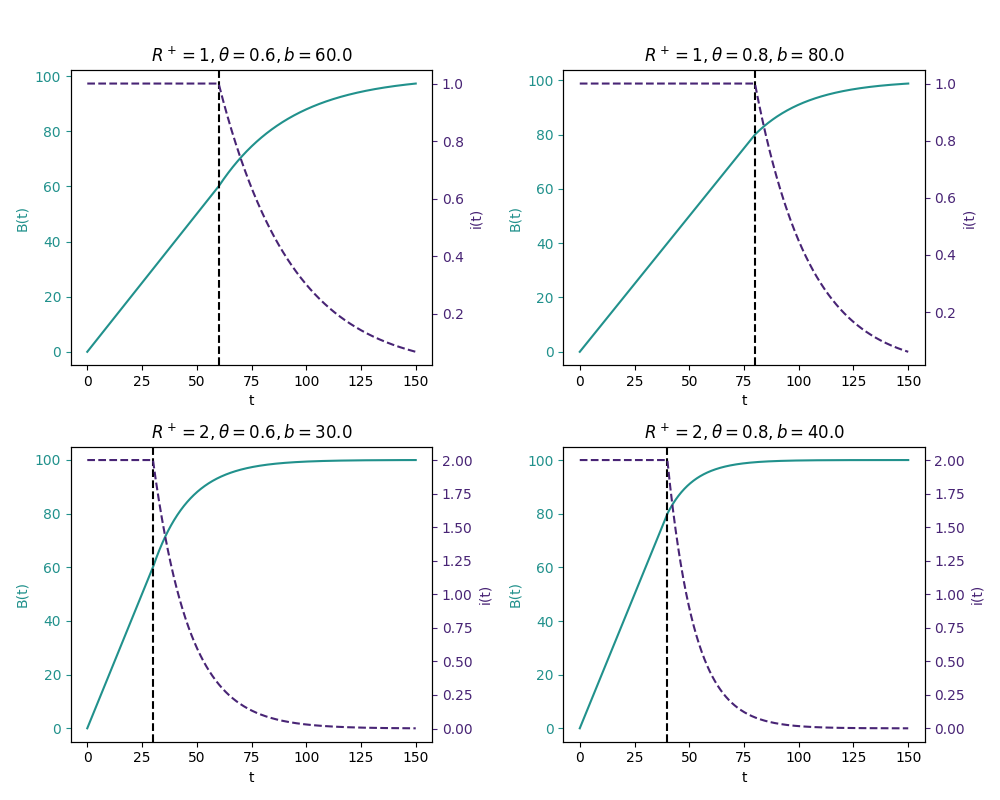
\includegraphics[width =12.5cm]{assets/img/07_graph_based/R_theta_combinations.png}
	\caption[Different Charging Profiles According To The Model]
	{Different charging profile obtained according to the model developed in \equaref{eq:cc_cv}. B is the State of Charge in Percentage, while $i(t)$ in function of the time unit $t$. The battery have $Q = 100$ %and the breakpoint is calculated as $b = \dfrac{Q\theta}{R^+}$  
	}
	\label{fig:charging_profiles}
\end{figure}
\begin{equation}
	B_a(t+1) = 
	\begin{cases} 
		%0 & \text{if } t+1 \leq 0 \\
		%B(t)_a + \int_{t}^{t+1} i(t)dt & \quad \text{if } t \leq  b_a\\
		B(t)_a + R^+_a & \quad \text{if } t \leq  b_a\\
		\\
		%R^+_a e^{-t+b_a} %& \text{else}
		Q_a - \dfrac{Q_ai(t)(1-\theta_a)}{R^+_a}
		\end{cases}
		\label{eq:cc_cv}
\end{equation}

with $b_a = \dfrac{\theta_a Q_a}{R^+_a}$,  $i(t)= \begin{cases} R^+_a \quad \text{if } t \leq  b_a\\
	R^+_a e^{-(t-b_a)/\tau}\\ \end{cases}$ and $\tau= \dfrac{C_n}{R^+_a\theta_a}\in \mathbb{R}_{\ge0}$  representing how quickly the current decreases. The value of $C_n$ depends on the charging device considered.   \\
	An example of the charging profiles from this model can be seen in \figref{fig:charging_profiles}. 
	 Since $i(t)$ is assumed to be constant at time $t\leq b_a$, i.e. $i(t) = R^+_a$,the first condition is derived as follows. 
\begin{align*}
	B_a(t+\alpha) &= B_a(t) + \int_{t}^{t+\alpha}R^+_adt\\
	B_a(t+\alpha) &= B_a(t) +R^+_a \int_{t}^{t+\alpha}dt\\
	B_a(t+\alpha) &= B_a(t) +R^+_a \quad t \bigg|_{t}^{t+\alpha}\\
	B_a(t+\alpha) &= B_a(t) +R^+_a (t+\alpha - t)\\
	B_a(t+\alpha) &= B_a(t) +\alpha R^+_a\\
\end{align*}
with $\alpha = 1$. \\
The discharging, on the other hand, will be modeled as it being directly proportional to the travel time $T$, as described in \equaref{eq:discharging}. 
%\begin{equation}
%	B_a(t+1) = B(t)_a - R^-_a ( \gamma d_a + (1-\gamma)T_a)
%	\label{eq:discharging}
%\end{equation} 
%where $\gamma \in [0,1]$. \\
\begin{equation}
	B_a(t+T_{u,v}^a) = B(t)_a - R^-_a T_{u,v}^a
	\label{eq:discharging}
\end{equation} 
The equation describes the relationship between the initial and final battery levels on edge $\langle v_u, v_v \rangle$ during the transit. Following \equaref{eq:discharging}, one can assign to each edge a rate of battery discharge by defining it as the difference between the state of charge at time $t$ and at time $t+T_{u,v}^a$. \\
\begin{equation}
	 e^a_{u,v} = B(t)_a - B_a(t+T_{u,v}^a) =  R^-_a T_{u,v}^a
	\label{eq:discharging_rate_per_edge}
\end{equation} 
\equaref{eq:discharging_rate_per_edge} allows to describe the discharging rate as a function of only the edge and the vehicle. \\
In terms of operational costs, multiple factors should be considered and the analysis must be extended from the one developed in \cite{project_thesis}, where the operational cost was only in function of the vehicle type. Similarly to the aforementioned work, this model assumes a certain operational cost depending on the vehicle type, however the discussion is also extended in terms of vehicle charging cost. In other words, we can decouple it from the general concept of the operational cost per vehicle and considering in function of the charging or discharging profiles described above. Furthermore, it also makes sense to assign the cost also depending on the distance traveled, i.e. the value $d$ associated to the edges. \\
Compared to \cite{project_thesis}, in this work, the model also extends the information associated to the nodes. Nodes will be of two categories namely normal nodes and charging (or depot) stations, whose sets are denoted as $\mathcal{V}_n$, $\mathcal{V}_c$, respectively. We can, therefore, conclude that $\mathcal{V} = \mathcal{V}_n \cup \mathcal{V}_c$. The information associated to the nodes depend from the category each node belongs to. Nodes belonging to $\mathcal{V}_n$ do not possess any specific information, as they are not of high importance for this work. Charging nodes $\mathcal{V}_c$, on the other hand, possess two main characteristics, namely their capacity and their charging ability. Intuitively, the term capacity is used to refer to the number of avilable parking spots, identified as $z_v$. Furthermore, three types of charging ability will be considered, i.e. fast, normal and slow charging, which will be based on the model in \equaref{eq:cc_cv}. The choice of parameters is explained in \tabref{tab:charging_stations}. 
\begin{table}[th]
	\centering
\begin{tabular}{ |p{2cm}|p{1cm}|p{1cm}|p{1cm}|p{1cm}|}
	\hline
	Type&$C_n$  &$\tau$&$\theta_a$&$R^+_a$ \\
	\hline
	Slow & 20 &$33.\bar{3}$&1&0.6  \\
	Medium &15 &18.17& 1   & 0.8\\
	Fast & 10 & 6.25&2& 0.8\\
	\hline
\end{tabular}
	\caption[Parameters choice for the Chargin Stations]{Choice of parameters for the charging stations according to the type. For the charging profile, please refer to \figref{fig:charging_profiles}. The first column is the costant related to the charging type, the second is the $\tau= \dfrac{C_n}{R^+_a\theta_a}\in \mathbb{R}_{\ge0}$ calculated with the values on the third and fourth column. }
	\label{tab:charging_stations}	
\end{table}\\

It is a sensible choice to limit the domain of the starting and terminal node of each vehicle to the sets of charging and depot nodes, i.e. $\underline{s_a}\in\mathcal{V}_c \cup \mathcal{V}_d \text{ and } \bar{t_a}\in \mathcal{V}_c \cup \mathcal{V}_d$. In other words, this choice implies that each vehicle's destination will either be the depot at the end of the shift, for example, or a charging node, where its battery can be charged to accomodate future requests. \\
Requests are modeled as tuples $\langle \underline{s'},\bar{t'}, G', P',\lambda, a', b'\rangle$, where  $\underline{s'} \in \mathcal{V}_n,\bar{t'} \in \mathcal{V}_n$ represent the pickup and delivery point respectively; $G'\in \mathbb{R}_{\ge0}$ ($P'\in \mathbb{R}_{\ge0}$) refers to the amount of goods (people) required to transport,  and $\lambda \in \mathbb{R}_{>0}$ is the rate of requests, in customers per unit time, which, therefore, makes the requests stationary and deterministic. Additionally, requests must be delivered within a time window within $[a',b']$. \\



\subsection{Model Evalutation}
Some comments are in order. The model in \secref{sec:vc_model} is time-invariant. According to the definition presented by \citepaperofs{amod_review}{Frazzoli}, time invariance in the context of transportation modeling refers to the assumption that the number of requests remain constant over time allowing for the simplification of temporal dynamics and treating specific time intervals as homogeneous units. This modeling concept is employed when the rate of change in transportation demands is deemed slow compared to the average travel time of individual trips, often observed in stable urban environments (\cite{neuburger1971}). While this model is indeed applied in a relatively dense urban environment, some integrations are required in order to adapt it to time-varying scenarios. Moreover, customer requests are also assumed to be known. This requirement can be fulfilled in practice with requests made in advance or some techniques to estimate requests throughout the day. It is important to note that request estimation might lead to suboptimal performance. \\
Secondly, as already mentioned in the previous section, the model used to describe congestions is indeed rather simple and more complex formulation might better capture the phenomena. However, the semplification is considered powerful enough for the purpose of this work and, as pointed out by \citepaperofs{congestion_vrp_phd_graph}{Zhang} as well, more sophisticated models can be used offline using simulation techniques to derive the capacity metric used in this model.\\
Some comments are in order also regarding vehicles. Firstly, we assume the vehicles to be autonomous and fault proof. It is outside of the scope of this work to deal malfunctioning vehicles or exceptional situations outside of the normale functioning regime of the system.Additionally, we assume the vehicles to be fully electric. This assumption is widely used in literature and it is motivated, among other aspects, also by the recent trends in industry to transition towards electrical mobility. Furthermore, the model provided for the battery charging and discharging profiles is rather simplistics and more sophisticated approaches exist in literature (see \chapref{ch:related_work} for more details). However, these models should be seen an addition to the corrent approach and, albeit with some potential modifications, it is plausible they can be integrated in the system model. While in \cite{project_thesis} vehicles have been designed to be capable of transporting a potentially large number of people, some considerations should be made in this regard. While it is sensitive to consider vehicles capable of transporting up to 50 people in terms of environmental, economical and overall transportation efficiency and while it is also expected that the model designed would work with those vehicles as well, in terms of practical use, it might be more appropriate to make use of those vehicles in different ways. Notably, it should be studied whether it is efficient to tailor the routes of those vehicles according to passenger needs. Firstly, if we do not consider ride-sharing possibilities, the scenario of such large group of people traveling together is very unlikely. Additionally, if we consider ride-sharing, the possible route combinations, which increases drastically as the number of requests and nodes in the graph increase, would likely make routing such vehicle relatively inefficient. Motivated also by the fact that passengers might have common stops, it might be more sensible to treat those vehicles as buses are treated nowadays, i.e. with a pre-determined route among stops which are placed according to the most common stops, such as hospitals or train stations. Similarly, if we consider large vehicles to transport goods, such as large trucks, those are not used for home delivery, but rather used to transport goods among specialized centers. It must be noted that both situations do not invalidate this work, or any previous work. It is clear that the system described in this work in combination to the truck for goods transportation. Regarding people mobility, while buses are indeed an already established and efficient transportation mean, this systems aims at filling up the situations where a bus system is indeed lacking, such as transportation of people with special needs or, in general, more tailored to the specific needs of potential customers. \\
In this model, we also made certain assumptions on the nodes. Firstly, there is no distinction between depot and charging nodes. The difference between charging and depot stations lays on the fact that charging nodes are not meant to host vehicles for long periods of time, contrary to depots. The difference can be envisioned as if charging stations were gas stations and depots were bus depots. The  model can be trivially extended according to this distinction. Additionally, it is assumed that the charging stations are all of the same types. It might be argued that some stations might have different types of chargers. This characteristics can be reflected by the model simply by 'splitting' them. A station having, for instance, two types of chargers can be represented by two equivalent nodes in the graph having different category. Moreover, while in \tabref{tab:charging_stations} we only considered three modes, this can be easily extended. 


\section{Problem Formulation}\label{sec:prob_form}
Before defining the problems for the different challenges faced by the AToD considered in this work, it is essential to lay down the motivations behind certain assumptions made during the conceptual phase. \\
Firstly, following the previously described model, it is assumed that each vehicle starts and ends at a charging or depot node, $\underline{s_a} \text{ and }\bar{t_a}$, which do not have to be necessarily the same. Furthermore, if a vehicle leaves from a depot, it is assumed to have a fully charged battery, i.e. $B_a(0) = 100$. 
%WE ASSUME THE CHARGE OF THE VEHICLE TO BE ENOUGH FOR ALL 
%REQUESTS, CHARGIN CAN ONLY BE DONE BEFORE REBALANCING, 
%THEREFORE WE ARE GOING TO LEAVE THIS PROBLEM TO ASSIGNMENT. 



\subsection{Dispatching}

\begin{figure}
	\begin{subfigure}{0.5\linewidth}
		\centering
		\begin{tikzpicture}
			% Nodes
			\node[draw, circle] (A) at (0,0) {A};
			\node[draw, circle] (B) at (2,0) {B};
			\node[draw, circle] (C) at (2,2) {C};
			\node[draw, circle] (D) at (0,2) {D};
			\node[draw, circle] (E) at (1,4) {E};
			
			% Directed edges
			\draw[->] (A) -- (B);
			\draw[->, red] (A) -- (C) node[midway,above,sloped] {
\includegraphics[width=0.5cm]{assets/img/07_graph_based/car.png} };
			\draw[->] (B) -- (C);
			\draw[->, red] (C) -- (D);
			\draw[->] (D) -- (A);
			\draw[->, black, dashed] ([yshift=2pt, xshift=-10]C.north) -- ([yshift=2pt, xshift=10pt]D.north);
			\draw[->, blue] (D) -- (E)node[midway,above,sloped] {
\includegraphics[width=0.5cm]{assets/img/07_graph_based/car.png} };
			\draw[->, blue] (E) -- (C);
		\end{tikzpicture}
		\caption{}
		\label{fig:req_assignable}
	\end{subfigure}%
	\begin{subfigure}{0.5\linewidth}
		\centering
		\begin{tikzpicture}
			% Nodes (duplicated)
			\node[draw, circle] (A) at (0,0) {A};
			\node[draw, circle] (B) at (2,0) {B};
			\node[draw, circle] (C) at (2,2) {C};
			\node[draw, circle] (D) at (0,2) {D};
			\node[draw, circle] (E) at (1,4) {E};
			
			% Directed edges (duplicated)
			\draw[->] (A) -- (B);
			\draw[->, red] (A) -- (C) node[midway,above,sloped] {
\includegraphics[width=0.5cm]{assets/img/07_graph_based/car.png} };
			\draw[->] (B) -- (C);
			\draw[->, black, dashed] ([yshift=2pt, xshift=10]D.north) -- ([yshift=2pt, xshift=-10pt]C.north);
			
			\draw[->, red] (C) -- (D);
			\draw[->] (D) -- (A);
			\draw[->, blue] (D) -- (E)node[midway,above,sloped] {
\includegraphics[width=0.5cm]{assets/img/07_graph_based/car.png} };
			\draw[->, blue] (E) -- (C);
		\end{tikzpicture}
		\caption{}
		\label{fig:req_notassignable}
	\end{subfigure}
	\caption[Example of a Sensible Request aAignment]{\figref{fig:req_assignable} and \figref{fig:req_notassignable} show a simplified example of a sensible request assignment. In red and blue are the paths the two AVs can traverse, while the dashed blue two different requests (In \figref{fig:req_assignable} the custoer asks to go from C to D, while in \figref{fig:req_notassignable} the customer asks to go from D to C). In the case of \figref{fig:req_assignable}, it is more sensible to assign the request to the red AV, while in the case of \figref{fig:req_notassignable}, the blue AV is a better choice. }
	\label{fig:sens_assignment}
\end{figure}

Informally, the dispatching problem can be defined as the task of assigning requests to the most suitable vehicle. There exist already multiple solutions proposed for the problem and we refer to \chapref{ch:related_work} for a more thorough analysis. \\
Dispatching is critical for the overall system performance and must be done in a way that can further facilitate the next steps. Clearly, dispatching can not be decoupled and solved as a stand-alone problem. For example, \figref{fig:sens_assignment} shows a simplified situation where a sensible dispatching, which depends on a posterior step, will improve system performance. Nevertheless, during the dispatching problem, some additional elements must be considered as well. \\
Since the model proposed in \secref{sec:vc_model} is a vehicle centric model, we can model the dispatching problem with the help of a binary variable $x_{ar}$ defined in \equaref{eq:dispatching_var}. 
\begin{equation*}
	x_{a,r} = 
	\begin{cases} 
		%0 & \text{if } t+1 \leq 0 \\
		%B(t)_a + \int_{t}^{t+1} i(t)dt & \quad \text{if } t \leq  b_a\\
		1 & \quad \text{if $r$ is assigned to } a \in \mathcal{A}\\
		\\
		%R^+_a e^{-t+b_a} %& \text{else}
		0
	\end{cases}
	\quad\quad \forall r \in \mathcal{R}
	\label{eq:dispatching_var}
\end{equation*}

According to the model, each vehicle has a capacity which must not be exceeded. Such constraint can be expressed as follows for both people and goods. 
\begin{align}
	\sum_{r \in \mathcal{R}} P_r' \cdot x_{a,r} &\leq P_a \quad \forall a \in \mathcal{A}\label{eq:cons_quantity_p}\\
	\sum_{r \in \mathcal{R}} G_r' \cdot x_{a,r} &\leq G_a \quad \forall a \in \mathcal{A}\label{eq:cons_quantity_g}
\end{align}
Furthermore, if a vehicle is already on the move, the request can be picked up only if the vehicle's charge is enough to satisfy such request as well. In this case, such requirement can be expressed as follows. 
\begin{equation}
	\sum_{r \in \mathcal{R}} e(\underline{s'_r}, \bar{t'_r}) x_{a,r}\leq B_a \quad \forall a \in \mathcal{A}\\
	\label{eq:cons_charg}
\end{equation}
where $e: \mathcal{E} \times \mathcal{E} \rightarrow \mathbb{R}_{>0}$ is a function expressing the required energy to go from $\underline{s'_r}$ to $\bar{t'_r}$.\\
Accordingly, using \equaref{eq:cons_quantity_p}, \ref{eq:cons_quantity_g}  and  \equaref{eq:cons_charg}, one can simply formulate it as an integer programming problem by finding the appropriate cost function to minimize, such as minimizing waiting times. Thanks to this formulation, one can also make sure that each request has been served at most $\lambda_r$ times , i.e. \equaref{eq:req_served}. 
\begin{equation}
	\sum_{a \in \mathcal{A}} x_{a,r} \leq \lambda_r \quad \forall r \in \mathcal{R}\\
	\label{eq:req_served}
\end{equation}
Furthermore, one must ensure that each request is assigned at most to one vehicle. This is expressed by \equaref{eq:req_served_per_vehicle}. 
\begin{equation}
	% \lambda_r
	\sum_{r \in \mathcal{R}} x_{a,r} \leq 1\quad \forall a \in \mathcal{A}\\
	\label{eq:req_served_per_vehicle}
\end{equation}
The above mentioned equations are based upon the work developed by \citepaperofs{hyland2018dynamic}{Hyland}. \\
This way allows to define the following cost function which expresses the number of served requests.
\begin{equation}
	\mathcal{J}_u = \sum_{r \in \mathcal{R}} (1  - \min_{a \in \mathcal{A}} (x_{a,r},1))\\
	\label{eq:req_unserved}
\end{equation}
 The main strength of this approach is that can be integrated naturally in the formulation for the other steps, like for e.g. the one in \secref{sec:routing}. \\
Alternatively, the dispatching problem can be solved independently without being integrated in other steps. For example, in \secref{ch:related_work}, some works are mentioned that make use of heuristics such as nearest neighbours. On the one hand,these approaches are known to obtain sub-optimal solutions for the problem; on the other hand, they provide flexibility and might result in less time or space complexity. \\


\subsection{Routing}\label{sec:routing}
After being assigned to incoming requests, vehicles must be routed in such a way that can reach all customers and therefore satisfy all the requests. In other words, the routing problem consists of determining paths, i.e. a series of edges, each vehicle must travel in the graph to fulfill the requests while respecting all the requirements and minimizing some metrics, i.e. a cost function. Since this problem can be reconduced to the
vehicle routing problem, in particular dynamic pickup and delivery problems (reviewd by \citepaperofs{TothPVigoD2014}{Toth} and \citepaperofs{LaporteG2009}{Laporte}), the formulation used in this work will be based on this family of problems. \\
Within our model, binary flow variables will be used to identify whether a vehicle should traverse a link. Formally, this can be expressed as 
\begin{equation*}
	V_{u,v}^a = 
	\begin{cases} 
		%0 & \text{if } t+1 \leq 0 \\
		%B(t)_a + \int_{t}^{t+1} i(t)dt & \quad \text{if } t \leq  b_a\\
		1 & \quad \text{if $a$ traverses } (u,v) \in \mathcal{E}\\
		\\
		%R^+_a e^{-t+b_a} %& \text{else}
		0
	\end{cases}
	\quad\quad \forall a \in \mathcal{A}, \forall u,v \in \mathcal{V}
	\label{eq:binary_edges}
\end{equation*}
Furthermore, another variable will be needed to deal with time-related requirements. This concept is based on the work in \cite{inbook_twvrp}. The decision variable $s_{u}^a$ indicates the service time of vehicle $a$ at node $u$. This  variable will be relevant only for nodes labeled as being terminal stations for the requests, i.e. $\underline{t'a}$ and will be irrelevant for other nodes. \\
Accordingly, one can express the abovementioned cost function using this variable. Classical examples of cost functions are for e.g. travel time and travel distance. These are frequently used in literature (\cite{7579135}), as they are general, in a sense that many other metrics could be reconducted to them. For example, residual charging or operational costs are directly influenced by the two. Furthermore, the formualtion of the cost function derived from these metrics is rather trivial and intuitive, while at the same time producing desirable results in practice. The formulation is described in equation \equaref{eq:travel_time_routing} and \ref{eq:distance_time_routing}. \\
\begin{align}
	\mathcal{J}_T = \sum_{a \in \mathcal{A}} &\sum_{(u, v) \in \mathcal{E}} T^a_{ u,v} V^a_{u,v} \label{eq:travel_time_routing}\\
	\mathcal{J}_d = \sum_{a \in \mathcal{A}} &\sum_{(u, v) \in \mathcal{E}} d_{ u,v} V^a_{u,v}\label{eq:distance_time_routing}
\end{align} 
In the effort to minimize the environmental impact of the AToD system, the pollution index discussed in previous sections can be utilized to formulate the cost function outlined in \equaref{eq:pollution_metric}.
\begin{equation}
	\mathcal{J}_f =\sum_{a \in \mathcal{A}} \sum_{(u, v) \in \mathcal{E}} f^a_{ u,v} V^a_{u,v} 
	\label{eq:pollution_metric}
\end{equation} 
Up to this point, the metrics under consideration have been geared towards minimization. Put differently, the goal is to reduce travel, encompassing both distance and time, to enhance system performance. Likewise, minimizing environmental impact is crucial in this scenario. However, there are instances where maintaining certain metrics at higher levels is preferable. For instance, closely tied to operational costs and environmental impact, it is advantageous to keep the state of charge at its maximum. Hence, it is imperative to maximize the cost function in Equation \ref{eq:soc_metric}.
\begin{equation}
	\mathcal{J}_B =\sum_{a \in \mathcal{A}}  B_a 
	\label{eq:soc_metric}
\end{equation} 
Finally, while it should also be explored whether the combination of those could improve the overall performance of the system. For this purpose, the cost functions can be combinated using weights as follows.  
\begin{equation}
	\mathcal{J}_{tot} = \lambda_T\mathcal{J}_T +\lambda_d\mathcal{J}_d +\lambda_f\mathcal{J}_f +\lambda_B\mathcal{J}_B 
	\label{eq:combined_metrics}
\end{equation} \\
where $\lambda_i \in \mathbb{R}$ with $i \in \{T, d,f, B\}$ are the weights.\\
It is not uncommon to also find in literature cost functions which are developed in terms of operational costs, as it provides a general idea to reason about this problem and allows for a systematic evaluation of different dispatching strategies. Moreover, the inclusion of operational costs in the literature emphasizes the real-world impact of dispatching decisions, aligning theoretical models with practical considerations. This connection to tangible costs not only enhances the applicability of proposed solutions but also contributes to the development of more realistic and effective dispatching strategies. Considering that, within our model in \secref{sec:vc_model}, each vehicle is modeled to have an operational cost, one can also derive a cost function similarly to what already done in \cite{project_thesis}. 
\subsubsection*{Unconstrained Version}
Before formulating the routing problem formally, a small consideration must be made. For convenience, the set of nodes recheable from node $u$ by traversing a single edge $\mathcal{N}^+_u$, i.e. the ingoing neighbours of $u$, and $\mathcal{N}^-_u$ as the set of outgoing neighbours of $u$.\\ Additionally, in order to ease the notation, the set containin all the initial stations of each request $r \in R_a$ will be indicated as $\underline{S_a'}$. Likewise,  $\bar{T_a'}$ will be the set of terminal stations of each request $r \in R_a$. \\
On a basic level, i.e. without constraints, one can formulate the \textit{Unconstrained Routing Problem (URP)} as follows. Given a transportation network $\mathcal{G}$, a set of vehicles $\mathcal{A}$ and a set of requests $\mathcal{R}$, defined within the description in section \secref{sec:vc_model}, solve:








\begin{align}
	\text{min}&  \text{
	(\ref{eq:travel_time_routing}), (\ref{eq:distance_time_routing}), (\ref{eq:pollution_metric}) or (\ref{eq:combined_metrics})
	}\nonumber\\
	\text{s.t.} &\nonumber\\
&\sum_{u \in \mathcal{V}} V^a_{u, v} - \sum_{w \in \mathcal{V}} V^a_{v, w} = 0 \quad \forall a \in \mathcal{A}, v \in \mathcal{V} \setminus \{\underline{s_a}, \bar{t_a}\} \label{eq:flow_conservation_graph_u} \\
&\sum_{ u \in \mathcal{N}^+_{\underline{s_a}} }V^a_{ \underline{s_a},u} = 1 \quad \forall a \in \mathcal{A} \label{eq:flow_cons_arrival_graph_u}\\
&\sum_{u \in \mathcal{N}^-_{\bar{t_a}} } V^a_{u, \bar{t_a}} = 1 \quad \forall a \in \mathcal{A} \label{eq:flow_cons_departure_graph_u}\\
%&\sum_{u \in \mathcal{V}} V^a_{u, v} - \sum_{w \in \mathcal{V}} V^a_{v, w} = 0 \quad \forall a \in \mathcal{A}, v \in \mathcal{V} \setminus ( \underline{S_a'} \cup \bar{T_a'})\label{eq:flow_conservation_graph2_u} \\
&\sum_{u \in \mathcal{N}^-_{\underline{t'_r}} } V^a_{u, \bar{t'_r}} = 1 \quad \forall r \in \bar{R_a}, \forall a \in \mathcal{A} 	\label{eq:flow_cons_arrival_graph_v_u}\\
&\sum_{u \in \mathcal{N}^+_{\underline{s'_r}} } V^a_{ \underline{s'_a},u} = 1 \quad \forall r \in \bar{R_a}, \forall a \in \mathcal{A}\label{eq:flow_cons_departure_graph_v_u}\\
&{p^a_u - p^a_v + P_a \cdot V_{u,v} \leq P_{a} - \sum_{r\in\mathcal{R}}P'_r, \quad \forall u, v \in \mathcal{V}, v \neq u, v \neq \underline{s}_a}\label{eq:no_sub_tour_g}\\
&{g^a_u - g^a_v + G_a \cdot V_{u,v} \leq G_{a} - \sum_{r\in\mathcal{R}}G'_r, \quad \forall u, v \in \mathcal{V}, v \neq u, v \neq \underline{s}_a}\label{eq:no_sub_tour_p}\\
&g^a_u \leq P_a;\quad p^a_u \leq P_a,   \quad\forall a \in \mathcal{A}\label{eq:final_req}\\
%& V^a_{u,\underline{s'_a}} \ge  V^a_{\bar{t'_a}, v} \quad \forall u\in \mathcal{N}^-_{\underline{s'_a}}, \forall v \in \mathcal{N}^+_{\bar{t'_a}} , \forall (\underline{s'_a}, \bar{t'_a}) \in R_a, \forall a \in \mathcal{A}\label{eq:s_before_t}
\nonumber
\end{align}



(\ref{eq:flow_conservation_graph_u}) insures that for all edges which do not lead to a source or destination, if $a$ reaches $v$ from a road, an incoming flow will lead to an outgoing one. In other words, they guarantee connections between roads. (\ref{eq:flow_cons_arrival_graph_u}) -  (\ref{eq:flow_cons_departure_graph_u}) insure that each universal source and destination is reached ones. Similarly, (\ref{eq:flow_cons_arrival_graph_v_u}) -  (\ref{eq:flow_cons_departure_graph_v_u}) achieves the same result, but for each requests.  It should be mentioned that to guarantee that those special nodes are reached at most once one can simply change from equalities to inequalites, like for e.g. $\sum_{ u \in \mathcal{N}^+_{\underline{s_a}} }V^a_{ \underline{s_a},u} \ge 1$.\\
Finally, (\ref{eq:no_sub_tour_g})-(\ref{eq:final_req}) assure that no sub-tour are presentes. This is inspired from the Miller-Tucker-Zemli formulation and utilizes two continuous decision variables $p^a, g^a \in \mathbb{R}_{\ge0}$ representing the cumulative load of the vehicle $a$. 

%Finally, (\ref{eq:s_before_t}) insures that source nodes are reached before the destinations. \\
In order to find the minimum number of vehicles required, one can use the method described \citepaperof{project_thesis}{Brodo}. 
\subsubsection*{Constrained Version}
While it could bring some interesting insights, the URP does not contain the necessary information to provide efficient routing for the scenario considered in this work. The goal is to identify the best possible path that \textup{(i)} satisfies all the requests and \textup{ii} is congestion free. The \textit{Congestion-Free Routing Problem (CRR)} is formally defined as follows.\\ Given a transportation network $\mathcal{G}$, a set of vehicles $\mathcal{A}$ and a set of requests $\mathcal{R}$, defined within the description in section \secref{sec:vc_model}, solve:

\begin{align}
	\text{min}&  
		(\ref{eq:travel_time_routing}), (\ref{eq:distance_time_routing}), (\ref{eq:pollution_metric}) \text{ or } (\ref{eq:combined_metrics})
	\nonumber\\
	\text{s.t.} &\nonumber\\
	&(\ref{eq:flow_conservation_graph_u})-(\ref{eq:flow_cons_departure_graph_v_u})\nonumber\\
	&\sum_{a \in \mathcal{A}}V^a_{u,v} \leq c_{u,v} \quad \forall (u,v) \in \mathcal{E} \label{eq:cong_free}\\
	&s_{u}^a + T_{u,v}^a - M*(1-V^a_{u,v}) \leq s_{v}^a  \quad \forall (u,v) \in \mathcal{E}, \forall a \in \mathcal{A}\label{eq:relations_node_time}\\
	%&V^a_{u,v}\cdot(s_{u}^a + T_{u,v}^a - s_{v}^a) \leq 0 \quad \forall (u,v) \in \mathcal{E}, \forall a \in \mathcal{A}\label{eq:relations_node_time}\\
	&a'_v \leq s_{v}^a \leq b'_v \quad \forall v \in \mathcal{E}, \forall a \in \mathcal{A}\label{eq:time_window_constraint}\\
	&\sum_{(u,v) \in \mathcal{E}}e^a_{u,v}\cdot V^a_{u,v} \leq B_a(0)\quad \forall a \in \mathcal{A} \label{eq:discharging_constraints}\\
	&M= \underset{(u,v) \in \mathcal{E}}{\text{max}}\{b_u + T_{u,v}-a_u\}\nonumber
\end{align} 
(\ref{eq:cong_free}) insures the number of vehicles in the link $(u,v)$ do not exceed the capacity of that link. (\ref{eq:relations_node_time}) establishes the relationship between the service time of each node, implying that the service time of a predecessor must be lower than the successor. (\ref{eq:time_window_constraint}) establish the time window constraints, indicating that it must be within the interval of the request. For nodes which are not associated with a termination node of a  request, one will simply set $a_v' = 0 $ and $b_a' = \infty$, also insuring that $s_v^a \ge 0 $. (\ref{eq:discharging_constraints}) assures that the vehicle charge is enough to cover all path. $B_a(0)$ can be assumed to be 100, i.e. that the batteries are full at the beginning of service. \\
In this formulation, the sub-tour elimination constraint is not required at it is already imposed by (\ref{eq:relations_node_time}). \\
\subsubsection*{Combination with Dispatching}
Multiple solutions have already been proposed in literature which solve the dispatching and routing problem in the same work. \\
In this work, however, in order to combine dispatching and routing into the same formulation, one must adapt some of the conditions specified in previous sections above. More specifically, each equation related to the requests must be changed to accomodate the fact that requests have not been previously assigned. \\
Accordingly, the \textit{Naive Routing and Dispatching Problem (NRDR)} can be formulated as 

\begin{align}
	\text{min}&  
		(\ref{eq:req_unserved}),
		(\ref{eq:travel_time_routing}), (\ref{eq:distance_time_routing}), (\ref{eq:pollution_metric}) \text{ or } (\ref{eq:combined_metrics})
	\nonumber\\
	\text{s.t.} &\nonumber\\
	&(\ref{eq:cons_quantity_p}),(\ref{eq:cons_quantity_g})\nonumber\\	
	&(\ref{eq:req_served}),(\ref{eq:req_served_per_vehicle})\nonumber\\	
	&(\ref{eq:flow_conservation_graph_u})\nonumber\\%-(\ref{eq:flow_cons_departure_graph_u})\nonumber\\
	&(\ref{eq:cong_free})-(\ref{eq:discharging_constraints})\nonumber\\
	&\sum_{ u \in \mathcal{N}^+_{\underline{s_a}} }V^a_{ \underline{s_a},u} = 1 \quad r \in \mathcal{R},  \forall a \in \mathcal{A} \label{eq:flow_cons_arrival_graph_u_d}\\
	&\sum_{u \in \mathcal{N}^-_{\bar{t_a}} } V^a_{u, \bar{t_a}} = 1 \quad r \in \mathcal{R},  \forall a \in \mathcal{A} \label{eq:flow_cons_departure_graph_u_d}\\
	&\sum_{u \in \mathcal{N}^-_{\underline{t'_r}} } V^a_{u, \bar{t'_r}} \ge x_{a,r} \quad  \forall r \in \mathcal{R}, \forall a \in \mathcal{A} \label{eq:must_arrive_dep}	\\
	&\sum_{u \in \mathcal{N}^+_{\underline{s'_r}} } V^a_{ \underline{s'_r}, u} \ge x_{a,r} \quad   \forall r \in \mathcal{R}, \forall a \in \mathcal{A}\label{eq:must_go_start}\\
	%&x_{a,r}\cdot(s_{\underline{s'_r}}^a - s_{\bar{t'_r}}^a) \leq 0 \quad \forall r \in \mathcal{R}, \forall a \in \mathcal{A}\label{eq:pick_bef_del}\\
	\nonumber
	%& V^a_{u,\underline{s'_a}} \ge  V^a_{\bar{t'_a}, v} \quad \forall u\in \mathcal{N}^-_{\underline{s'_a}}, \forall v \in \mathcal{N}^+_{\bar{t'_a}} , \forall (\underline{s'_a}, \bar{t'_a}) \in R_a, \forall a \in \mathcal{A}\label{eq:s_before_t}
\end{align}
Constraints (\ref{eq:flow_cons_arrival_graph_u_d}) and (\ref{eq:flow_cons_departure_graph_u_d}) impose that a vehicle must leave the starting depot and reach its final depot, respectively.  (\ref{eq:must_arrive_dep}) guarantees that, when a request $r$ is allocated to vehicle $a$, the vehicle must reach the terminal station of the request at least once. Moreover, equation (\ref{eq:must_go_start}) ensures that the vehicle traverses the starting station associated with the assigned request. \\
These requirements, furtermore, with this formulation, also ensure that a vehicle can only move from one node to the other only if they left the starting depot as well. \\ 
As an alternative to (\ref{eq:flow_cons_arrival_graph_u_d}) and (\ref{eq:flow_cons_departure_graph_u_d}), one can also relate the two constraints to the request assignment, which would transform the requirements as following. 
\begin{align}
	&\sum_{ u \in \mathcal{N}^+_{\underline{s_a}} }V^a_{ \underline{s_a},u} = \underset{ r \in \mathcal{R}}{\max}\{x_{a,r}\} \quad  \forall a \in \mathcal{A} \label{eq:flow_cons_arrival_graph_u_d2}\\
	&\sum_{u \in \mathcal{N}^-_{\bar{t_a}} } V^a_{u, \bar{t_a}} = \underset{ r \in \mathcal{R}}{\max}\{x_{a,r}\}  \quad r \in \mathcal{R},  \forall a \in \mathcal{A} \label{eq:flow_cons_departure_graph_u_d2}
\end{align}\\
In other words, a vehicle must leave the starting depot and reach the final depot if a request is assigned to it. \\
One can argue that the CRR can be reformulate to solve the dispatching in a different way. \\
Let 

\begin{equation*}
	x_{a,\underline{s_r} }= 
	\begin{cases} 
		%0 & \text{if } t+1 \leq 0 \\
		%B(t)_a + \int_{t}^{t+1} i(t)dt & \quad \text{if } t \leq  b_a\\
		1 & \quad \text{if $\underline{s_r} $ is reached by }  a \in \mathcal{A}\\
		\\
		%R^+_a e^{-t+b_a} %& \text{else}
		0
	\end{cases}
	\quad\quad \forall r \in \mathcal{R}
	\label{eq:var_dispatching}
\end{equation*}

 and given a transportation network $\mathcal{G}$, a set of vehicles $\mathcal{A}$ and a set of requests $\mathcal{R}$, defined within the description in section \secref{sec:vc_model}, solve:\\
\begin{align}
	\text{min}&  
		(\ref{eq:travel_time_routing}), (\ref{eq:distance_time_routing}), (\ref{eq:pollution_metric}) or (\ref{eq:combined_metrics})
	\nonumber\\
	\text{s.t.} &\nonumber\\
	&(\ref{eq:flow_conservation_graph_u})-(\ref{eq:flow_cons_departure_graph_u})\nonumber\\
	&(\ref{eq:cong_free})-(\ref{eq:discharging_constraints})\nonumber\\
	%&(\ref{eq:no_sub_tour_g})-(\ref{eq:final_req})\nonumber\\
	&\sum_{ a \in \mathcal{A} }
	\sum_{u \in \mathcal{N}^+_{\underline{s'_r}} } \alpha_a \cdot V^a_{ \underline{s'_r}, u} \ge \alpha'_r \quad \forall r \in \mathcal{R}, \forall \alpha \in \{G, P\}	\label{eq:leaving_from_starting_req}\\
	&\sum_{ a \in \mathcal{A} }\sum_{u \in \mathcal{N}^+_{\underline{s'_r}} } V^a_{ \underline{s'_r}, u} =\lambda_r\quad \forall r \in \mathcal{R}	\label{eq:each_request_ones}\\
	&\sum_{u \in \mathcal{N}^+_{\underline{s'_r}} }  V^a_{ \underline{s'_r}, u} \leq \sum_{u \in \mathcal{N}^-_{\bar{t'_r}} }  V^a_{u,\bar{t'_r}} \label{eq:first_start}
	%& V^a_{u,\underline{s'_a}} \ge  V^a_{\bar{t'_a}, v} \quad \forall u\in \mathcal{N}^-_{\underline{s'_a}}, \forall v \in \mathcal{N}^+_{\bar{t'_a}} , \forall (\underline{s'_a}, \bar{t'_a}) \in R_a, \forall a \in \mathcal{A}\label{eq:s_before_t}
\end{align}
(\ref{eq:leaving_from_starting_req}) insures that request can be served by the vehicle according to its capacity. (\ref{eq:each_request_ones}) guarantees each request is served $\lambda_r$ times and (\ref{eq:first_start}) insures that each vehicle reaches the terminal station of each request. 
\subsection{Rebalancing}\label{sec:rebal}
In simpler terms, the rebalancing problem revolves around efficiently redistributing autonomous vehicles (AVs) to optimize their responsiveness to new ride requests while minimizing any existing imbalances in the system. The goal is to fine-tune the positioning of AVs, ensuring they are strategically placed to promptly meet user demands and address any inherent irregularities in the distribution of service requests. This challenge is particularly crucial in ride-sharing  systems and transportation systems alike, where the dynamic nature of user requests and varying demand across different locations can lead to imbalances in the fleet's distribution. Effectively tackling the rebalancing problem enhances the overall efficiency of the system, providing users with quicker response times and a more evenly distributed service, ultimately contributing to a smoother and more reliable autonomous transportation network. \\
The formulation of the rebalancing problem is partially inspired from the works of \citepaperofs{congestion_vrp_phd_graph}{Zhang} and \citepaperofs{8593743}{Wallar}.  \\
The model previosuly described allows to reason on the rebalancing model in a novel manner when compared to the literature reviewed in \chapref{ch:related_work}. More specifically one could deal with the rebalancing by leveraging the request arrival rate $\lambda_r$ and the fact that vehicles are assumed to have a starting and terminal station, $\underline{s_a}$ and $\bar{t_a}$ respectively. \\

\begin{figure}
	\centering
	\begin{tikzpicture}[>=Stealth, node distance=2cm]
		
		% Draw rectangle
		\draw (-1,0) rectangle (8,4);
		
		% Nodes
		\foreach \x/\y/\n in {0/1/A, 3.5/1/B, 7/1/C,  0/3/G, 3.5/3/H, 7/3/I} {
			\node[dashed, circle, draw, fill=white] (\n) at (\x, \y) {$\n$};
		}
		
		\foreach \x/\y/\n in { 0.5/2/D, 3/2/E, 6/2/F} {
			\node[circle, draw, fill=white] (\n) at (\x, \y) {$\n$};
		}
		

		% Groups
		\draw[dashed, fill=red, fill opacity=0.2] (-0.5,0.5) rectangle (2,3.5);
		\draw[dashed, fill=blue, fill opacity=0.2] (2,0.5) rectangle (5,3.5);
		\draw[dashed, fill=green, fill opacity=0.2] (5,0.5) rectangle (7.5,3.5);
		
		% Arrows
		\foreach \from/\to in {A/B, B/C, D/E, E/F, G/H, H/I, A/D, B/E, C/F, D/G, E/H, F/I, G/B, H/C, I/E} {
			\draw[->] (\from) -- (\to);
		}
	\end{tikzpicture}
	\caption[Simplified Example for the Rebalancing Strategy]{Simplfied example for the rebalancing strategy.  Nodes D, E, F (continuos circles) to be the depot (or charging stations), while the other nodes (dashed circles) to be normal nodes. The graph has been previously divided in three areas (red, blue and green).  }
	\label{fig:division_graph}
\end{figure}
Considering the situation depicted in \figref{fig:division_graph} with a set of requests $\mathcal{R}'$ and a sets of vehicles $\mathcal{A}'$. According to this example, the graph is contained within the space $\Omega$, which has been divided in three cells (in red, blue and green). This division has been done arbitrarily in this case, but different strategies can be used (\cite{8593743}, \cite{voronoi_part}). These regions must be specified, however, in such a way that they contain exactly one node belonging to $\mathcal{V}_c$ and more than $n \in \mathbb{Z}_{\ge 1}$ nodes belonging to $\mathcal{V}_n$. Informally, this means that those regions are build around each charging station or depot and contain a certain amount of normal nodes. Different strategies could be used to determin this amount, like for e.g. all the nodes within a radius $r$ from each terminal node or within a driving distance $T_{max}$. Nevertheless, as a result of this, one will obtain a set of regions $R$. Formally, each region around a node $v \in \mathcal{V}_c$ can be defined as a subgraph $\mathcal{G}_v = \langle \mathcal{V}'_v, \mathcal{E}'_v\rangle$, where  \\
\begin{align}
\mathcal{V}_v' &= \{ u \in \mathcal{V}_n : (u, v) \in \mathcal{E} \wedge (v, u) \in \mathcal{E} , f(v,u) = 1 \} \cup \{ v\} \label{eq:v_prim_def}\\
\mathcal{E}'_v &= \{ (u, w) \in \mathcal{E} : u, w \in \mathcal{V}' \} 
\end{align}
In (\ref{eq:v_prim_def}), the function $f :  \mathcal{V}_c \times \mathcal{V}_n \rightarrow \{0,1\}$ is used to establish whether a node $u$ belongs to the region of $v$ ($f(v,u) = 1$) or not ($f(v,u) = 0$), as discussed before. Accordingly, one can obtain the total number of requests of region $v$ ($|\mathcal{R}'_v|$) by considering the requests which have a terminal node in $\mathcal{V}_n$. In other words
\begin{equation}
|\mathcal{R}'_v| = \sum_{r \in \mathcal{R}_v'} \lambda_r
\end{equation}
where 
\begin{equation}
\mathcal{R}_v'= \{ r \in \mathcal{R} : \underline{s_r}' \in \mathcal{V'}_v \} \label{eq:req_per_reg}
\end{equation}
In simple words, the set of $\mathcal{R}_v'$ indicates all the requests that start within the region of the node $v \in \mathcal{V}_c$. \\
Analogally, one can provide an alternative definition for $\mathcal{R}_v'$ in terms of the terminal station $u$.
\begin{equation}
	\mathcal{R}_u'= \{ r \in \mathcal{R} : \bar{t_r}' = u \}%\in \mathcal{V'}_v \} 
\end{equation}
Requests, therefore, are distributed over those regions and it is not hard to envision scenarios where requests are unequally distributed, i.e. regions with a higher $|\mathcal{R}^v| $ than others. As a result, due to the heterogenous nature of the nodes and the requests, AToD might experience imbalance, as AVs can be scattered through the whole graph if requests have different terminal nodes. Conversely, the opposite might happen, if all the requests have the same terminal node, but start from different areas. \\ 
Assuming all the requests in $\mathcal{R}'$ to be served, each vehicle's starting position is now either D, E, or F, i.e. $\underline{s_a} \in \{D, E, F\} \quad \forall a \in \mathcal{A}'$. This is due to the fact that, according to the transportation network model, since the requests have all been served, the vehicles have all reached their previous ending stations $\bar{t}_a$, which became their new starting nodes. \\
As a result, the solution of the rebalancing problem becomes ensuring that there is a sufficient number of vehicles at the depot (or charging) nodes to fulfill as many requests as possible in the given area, potentially covering all requests.
%. Assuming, within set of requests $\mathcal{R}'$, a set of terminal nodes  $\bar{T_r}$ and a set of rates $\Lambda$. \\

\subsubsection*{Unconstrained Rebalancing Problem}
To formulate the different versions of the rebalancing problem binary flow variables will be introduced to help with the different formulations. Similarly to \secref{sec:routing}, those variables will be useed to indicate whether an idle vehicle, i.e. a vehicle not currently transporting customers or goods, should be moving from a node to another. Formally, this is expresseed as follows. 
\begin{equation*}
	y_{u,v}^a = 
	\begin{cases} 
		%0 & \text{if } t+1 \leq 0 \\
		%B(t)_a + \int_{t}^{t+1} i(t)dt & \quad \text{if } t \leq  b_a\\
		1 & \quad \text{if $a$ traverses } (u,v) \in \mathcal{E}\\
		\\
		%R^+_a e^{-t+b_a} %& \text{else}
		0
	\end{cases}
	\quad\quad \forall a \in \mathcal{A}, \forall u,v \in \mathcal{V}
	\label{eq:binary_edges_reb}
\end{equation*}
Within the assumptions made at the beginning of this section, it follows that a vehicle will be considered idle if it is currently at its final station. \\
For the sake of simplicity and brevity, a generic cost function $\mathcal{J'}$ will be considered for the entirity of this section since the choice of a cost function is similar to the one for \secref{sec:vc_model}. \\
Finally, within the model established in prior sections, the \textit{Unconstrained Rebalancing Problem (UReP)} can be formulated as following. \\
Given a transportation network $\mathcal{G}$, a set of idle vehicles $\mathcal{A'}$ and a set of nodes belonging to $ \mathcal{V}_c$, defined within the description in section \secref{sec:vc_model}, solve:
\begin{align}
	\text{min}&  \quad \mathcal{J'} \nonumber \\
	\text{s.t.} &\nonumber\\
	&\sum_{u \in \mathcal{V}} y^a_{u, v} - \sum_{w \in \mathcal{V}} y^a_{v, w} = 0 \quad \forall a \in \mathcal{A'}, v \in \mathcal{V} \setminus \{\underline{s_a}, \bar{t_a}\} \label{eq:flow_conservation_graph_u23} \\	
	&\sum_{ u \in \mathcal{N}^+_{\underline{s_a}} }y^a_{ \underline{s_a},u} = 1 \quad \forall a \in \mathcal{A'} \label{eq:each_vehicle_start}\\
	&\sum_{\bar{t} \in \mathcal{V}_c}\sum_{ u \in \mathcal{N}^-_{\bar{t}} }y^a_{u, \bar{t}} = 1 \quad \forall a \in \mathcal{A'},  \label{eq:each_vehicle_end}\\
	&\sum_{a \in \mathcal{A'}}\sum_{u \in \mathcal{N}^-_{\bar{t}} } y^a_{u, \bar{t}} \leq z_{\bar{t}} \quad \forall \bar{t} \in \mathcal{V}_c \label{eq:capacity_depot_respected}\\
	&\sum_{a \in \mathcal{A'}}\sum_{u \in \mathcal{N}^-_{\bar{t}} } G_a \cdot y^a_{u, \bar{t}} \ge \sum_{r \in \mathcal{R'}_{\bar{t}}} G'_r \quad \forall \bar{t} \in \mathcal{V}_c \label{eq:goods_cap}\\
	&\sum_{a \in \mathcal{A'}}\sum_{u \in \mathcal{N}^-_{\bar{t}} } P_a \cdot y^a_{u, \bar{t}} \ge \sum_{r \in \mathcal{R'}_{\bar{t}}} P'_r \quad \forall \bar{t} \in \mathcal{V}_c \label{eq:people_cap}\\
	%&\sum_{u \in \mathcal{N}^+_{\underline{t'_a}} } V^a_{u, \bar{t'_a}} = 1 \quad \forall \bar{t'_a} \in \bar{T_a'}, \forall a \in \mathcal{A} 	\label{eq:flow_cons_arrival_graph_v_u}\\
	%&\sum_{u \in \mathcal{N}^+_{\underline{s'_a}} } V^a_{u, \underline{s'_a}} = 1 \quad \forall \underline{s'_a} \in \underline{S_a'}, \forall a \in \mathcal{A}\label{eq:flow_cons_departure_graph_v_u} \\
	\nonumber%
\end{align}
(\ref{eq:flow_conservation_graph_u23}) insures the flow conservation. (\ref{eq:each_vehicle_start}) indicates that the vehicles leave the starting node only from one edge. (\ref{eq:each_vehicle_end}) guarantees a vehicle must reach only one deposit at the time. (\ref{eq:capacity_depot_respected}) insures there the capacity of the deposits is respected. Finally, (\ref{eq:goods_cap}) and (\ref{eq:people_cap}) are used to ensure the vehicles being rebalanced to a certain station have the capacity to fulfill the requests of the area. 

\subsection{Constrained Congestion-Free Routing and Rebalancing Problem}
The final \textit{Constrained Congestion-Free Routing and Rebalancing Problem (CCRRP)} can be formulated as follows. \\
Given a transportation network $\mathcal{G}$, a set of vehicles $\mathcal{A}$, a set of total requests $\mathcal{R}$ and the sets of requests per region $\mathcal{R}'$ (\equaref{eq:req_per_reg}), solve: \\

\begin{align}
	\text{min}&  
		(\ref{eq:travel_time_routing}), (\ref{eq:distance_time_routing}) \text{ or } (\ref{eq:pollution_metric})
	\nonumber\\
	\text{s.t.} &\nonumber\\
	&(\ref{eq:flow_conservation_graph_u})-(\ref{eq:flow_cons_arrival_graph_u})\nonumber\\
	&(\ref{eq:leaving_from_starting_req})-(\ref{eq:first_start})	\nonumber\\
	&(\ref{eq:relations_node_time})-(\ref{eq:discharging_constraints})\nonumber\\
	%&(\ref{eq:no_sub_tour_g})-(\ref{eq:final_req})\nonumber\\
	&\sum_{\bar{t} \in \mathcal{V}_c}\sum_{ u \in \mathcal{N}^-_{\bar{t}} }V^a_{u, \bar{t}} = 1 \quad \forall a \in \mathcal{A},  \label{eq:each_vehicle_end2}\\
	&\sum_{a \in \mathcal{A}}\sum_{u \in \mathcal{N}^-_{\bar{t}} } V^a_{u, \bar{t}} \leq z_{\bar{t}} \quad \forall \bar{t} \in \mathcal{V}_c \label{eq:capacity_depot_respected2}\\
	&\sum_{a \in \mathcal{A}}\sum_{u \in \mathcal{N}^-_{\bar{t}} } G_a \cdot V^a_{u, \bar{t}} \ge \sum_{r \in \mathcal{R'}_{\bar{t}}} G'_r \quad \forall \bar{t} \in \mathcal{V}_c \label{eq:goods_cap2}\\
	&\sum_{a \in \mathcal{A}}\sum_{u \in \mathcal{N}^-_{\bar{t}} } P_a \cdot V^a_{u, \bar{t}} \ge \sum_{r \in \mathcal{R'}_{\bar{t}}} P'_r \quad \forall \bar{t} \in \mathcal{V}_c \label{eq:people_cap2}\\
	%&\text{(\ref{eq:flow_conservation_graph_u23})-(\ref{eq:people_cap})}\nonumber\\
	%&\sum_{(u,v) \in \mathcal{E}}e^a_{u,v}\cdot (V^a_{u,v} + y^a_{u,v}) \leq B_a(0)\quad \forall a \in \mathcal{A} \label{eq:discharging_constraints2}\\
	%&\sum_{a \in \mathcal{A}}(V^a_{u,v} + y^a_{u,v}) \leq c_{u,v} \quad \forall (u,v) \in \mathcal{E} \label{eq:cong_free2}\\
	%&V^a_{u,v} + y^a_{u,v} \leq 1 \quad \forall (u,v) \in \mathcal{E}, \forall a \in \mathcal{A} \label{eq:either_one_or_the_other}
\end{align}
Critically, compared to most of the reviewed literature, the strength of this approach lies in the fact that the rebalancing problem resembles more an assignment problem than routing. As a matter of fact, vehicles are routed in such a way that all the requests are guaranteed to be served and at the same time, the inbalance nature of AToD systems is tackled by ensuring that each region has enough vehicle to deal with future requests. \\
Furthermore, due to its vehicle-centric approach, this formulation offers significant flexibility across several dimensions: (i) it accommodates diverse request types, such as goods or people, (ii) it allows for a wide range of vehicle characteristics and specification, like for e.g. different capacities or dischargin profiles, and (iii) it remains adaptable to various node characteristics, as nodes have different number parking spaces, for example. Simultaneously, it exhibits scalability, with the number of variables increasing linearly in relation to the edges in the graph and the number of vehicles under consideration.
%
%\begin{align}
%	\text{minimize} \quad &\sum_{a \in \mathcal{A}} \sum_{(u, v) \in \mathcal{E}} T^a_{ u,v} x^a_{u,v} \label{eq:cost_graph}\\
%	\text{subject to} &\sum_{u \in \mathcal{V}} x^a_{u, v} - \sum_{w \in \mathcal{V}} x^a_{v, w} = 0 \quad \forall a \in \mathcal{A}, v \in \mathcal{V} \setminus \{\underline{s_a}, \bar{t_a}\} \label{eq:flow_conservation_graph} \\
%	&\sum_{ u \in \mathcal{V}\setminus \{\underline{s_a}\}} x^a_{ \underline{s_a},u} = 1 \quad \forall a \in \mathcal{A} \\
%	&\sum_{u \in \mathcal{V}\setminus \{ \bar{t_a}\} } x^a_{u, \bar{t_a}} = 1 \quad \forall a \in \mathcal{A} \label{eq:flow_cons_arrival_graph}\\
%	&\sum_{u \in \mathcal{V}\setminus \{ \bar{t'_a}\} } x^a_{u, \bar{t'_a}} = 1 \quad \forall \bar{t'_a} \in R_a, \forall a \in \mathcal{A} 	\\
%	&\sum_{u \in \mathcal{V}\setminus \{ \underline{s'_a}\} } x^a_{u, \underline{s'_a}} = 1 \quad \forall \underline{s'_a} \in R_a, \forall a \in \mathcal{A} \\
%	& \sum_{a \in \mathcal{A}}x^a_{u,v} \leq c_{u,v} \quad \forall (u,v) \in \mathcal{E}\\
%\end{align}
%
%


%\begin{align}
%	\text{minimize} & \quad (\text{\ref{eq:travel_time_routing}}, \text{\ref{eq:distance_time_routing}}, \text{\ref{eq:pollution_metric}} \text{ or } \text{\ref{eq:combined_metrics}}) \nonumber \\
%	\text{subject to} & \nonumber \\
%	& \sum_{u \in \mathcal{V}} V^a_{u, v} - \sum_{w \in \mathcal{V}} V^a_{v, w} = 0 \quad \forall a \in \mathcal{A}, v \in \mathcal{V} \setminus \{\underline{s_a}, \bar{t_a}\} \label{eq:flow_conservation_graph_u} \\
%	& \sum_{u \in \mathcal{N}^+_{\underline{s_a}}} V^a_{\underline{s_a}, u} = 1 \quad \forall a \in \mathcal{A} \label{eq:flow_cons_arrival_graph_u} \\
%	& \sum_{u \in \mathcal{N}^+_{\bar{t_a}}} V^a_{u, \bar{t_a}} = 1 \quad \forall a \in \mathcal{A} \label{eq:flow_cons_departure_graph_u} \\
%	& \sum_{u \in \mathcal{N}^+_{\underline{t'_a}}} V^a_{u, \bar{t'_a}} = 1 \quad \forall \bar{t'_a} \in \bar{T_a'}, \forall a \in \mathcal{A} \label{eq:flow_cons_arrival_graph_v_u} \\
%	& \sum_{u \in \mathcal{N}^+_{\underline{s'_a}}} V^a_{u, \underline{s'_a}} = 1 \quad \forall \underline{s'_a} \in \underline{S_a'}, \forall a \in \mathcal{A} \label{eq:flow_cons_departure_graph_v_u} \\
%	& \sum_{a \in \mathcal{A}} x_{ar} = 1 \quad \forall r \in \mathcal{R} \label{eq:request_assignment} \\
%	& \sum_{r \in \mathcal{R}} x_{ar} \leq 1 \quad \forall a \in \mathcal{A} \label{eq:vehicle_assignment_limit} \\
%	& V^a_{u, v}, x_{ar} \in \{0, 1\} \quad \forall a \in \mathcal{A}, \forall u, v \in \mathcal{V}, \forall r \in \mathcal{R} \nonumber
%\end{align}
\section{Use Case}
\begin{figure}[tbh]
	\centering
	\begin{subfigure}[b]{0.32\textwidth}
		\centering
		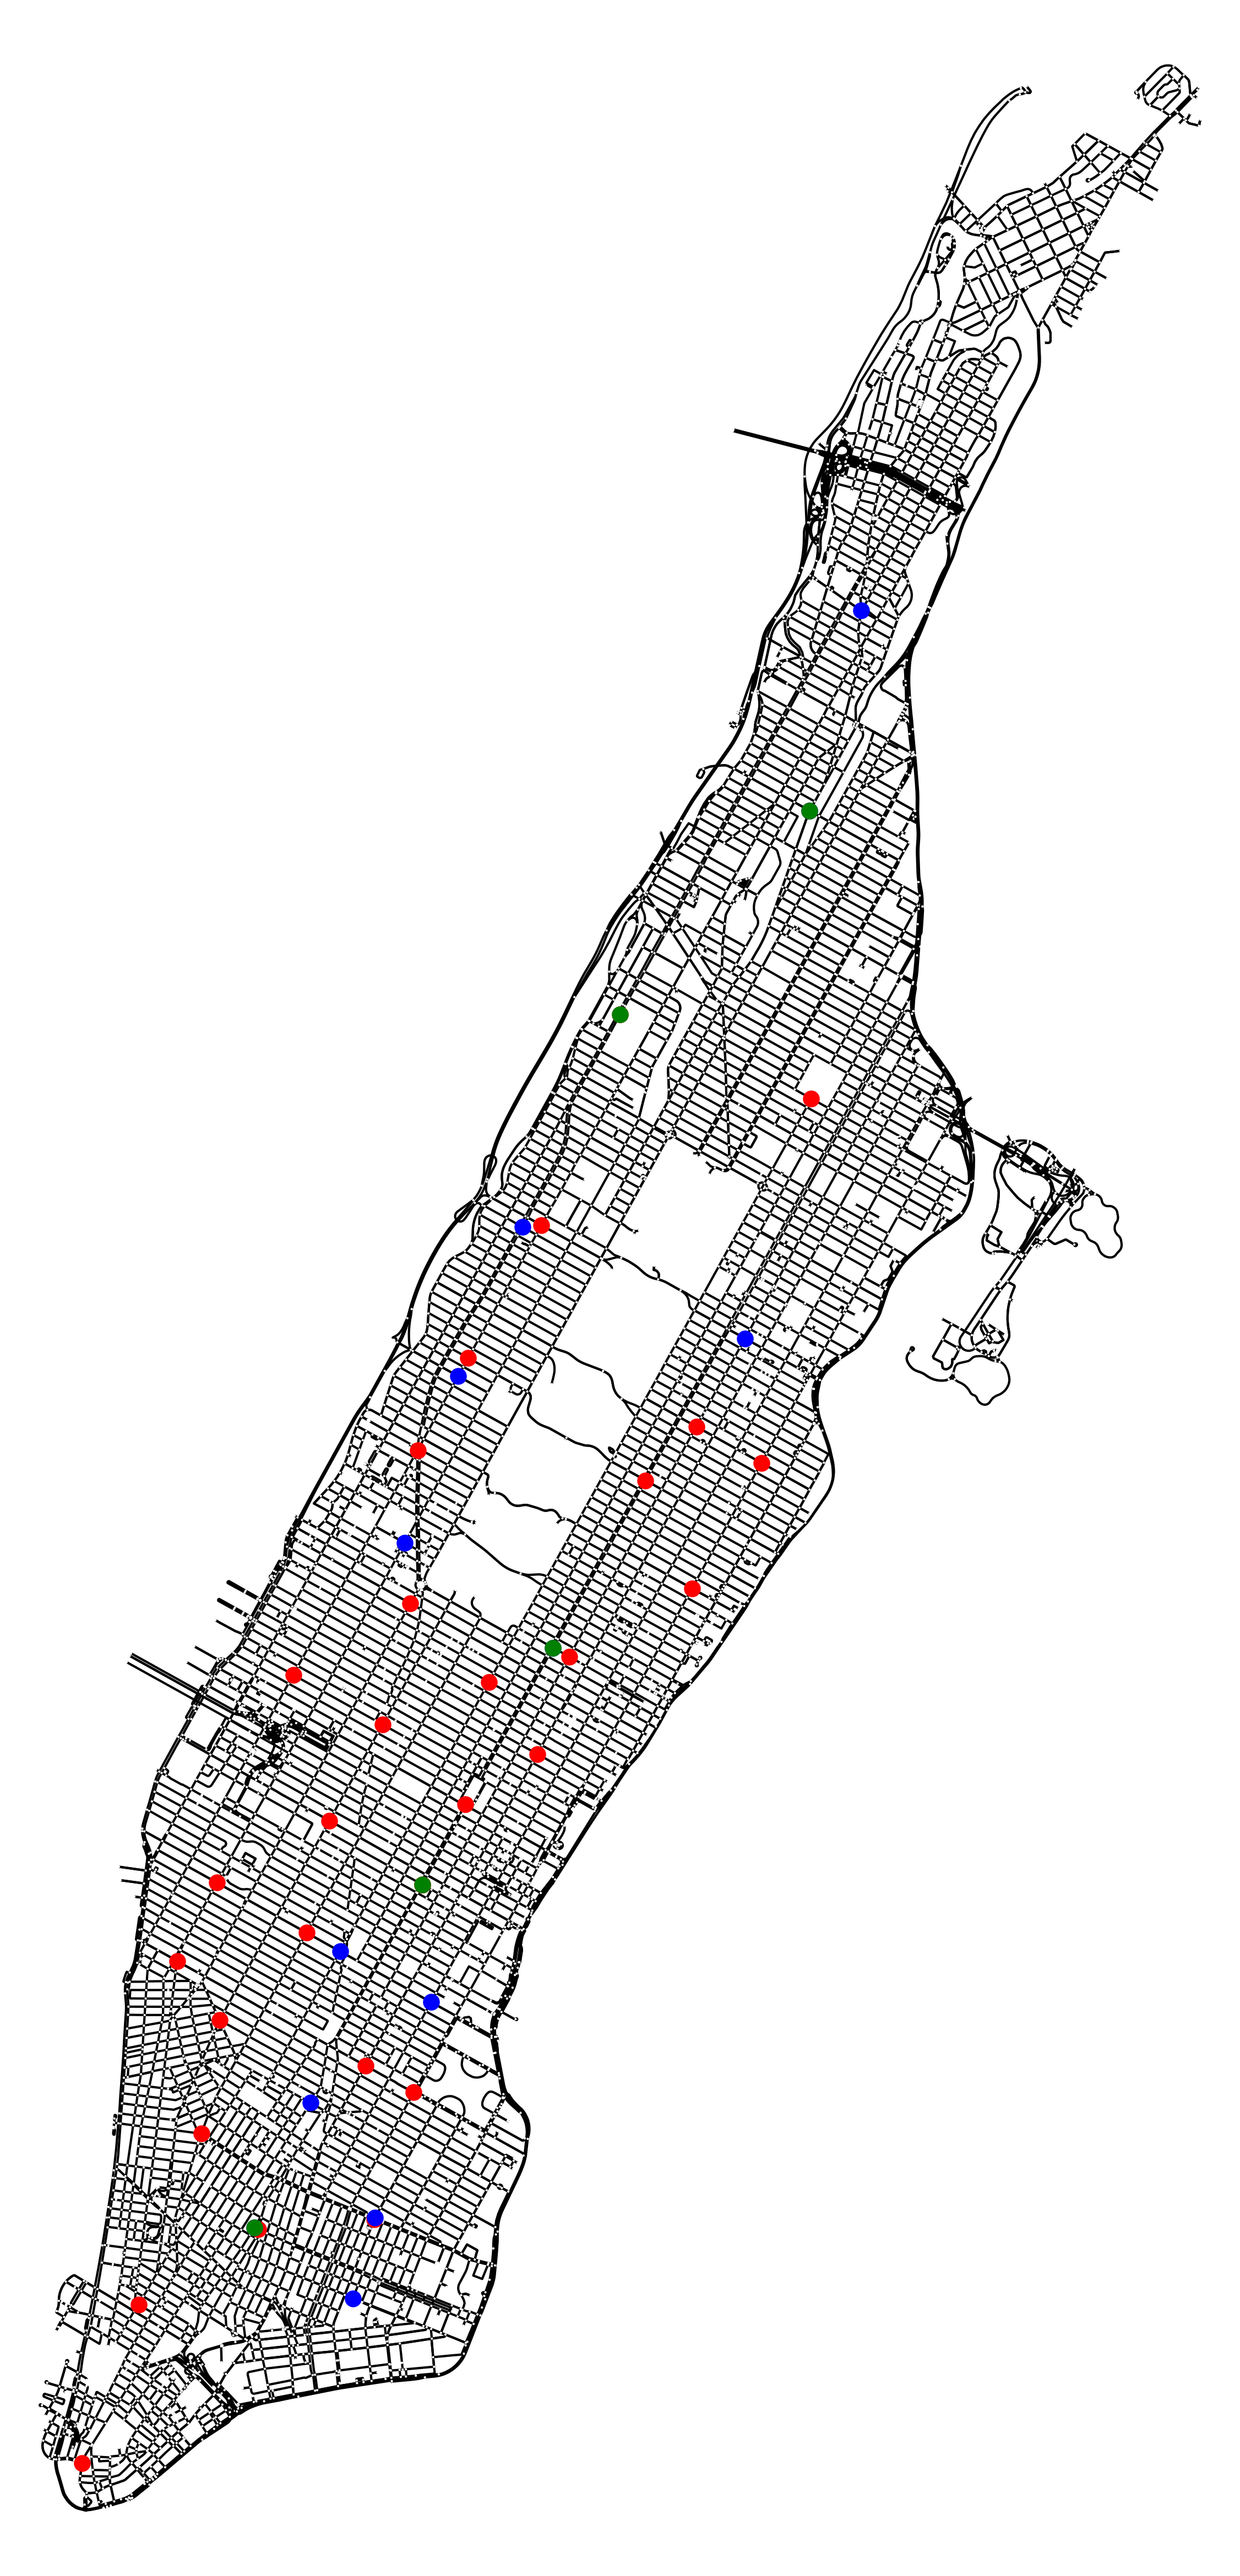
\includegraphics[width=\textwidth]{assets/img/07_graph_based/new_york_vanilla_info.png}
		\caption{}
		\label{fig:nyc_rn_info}
	\end{subfigure}
	\begin{subfigure}[b]{0.32\textwidth}
		\centering
		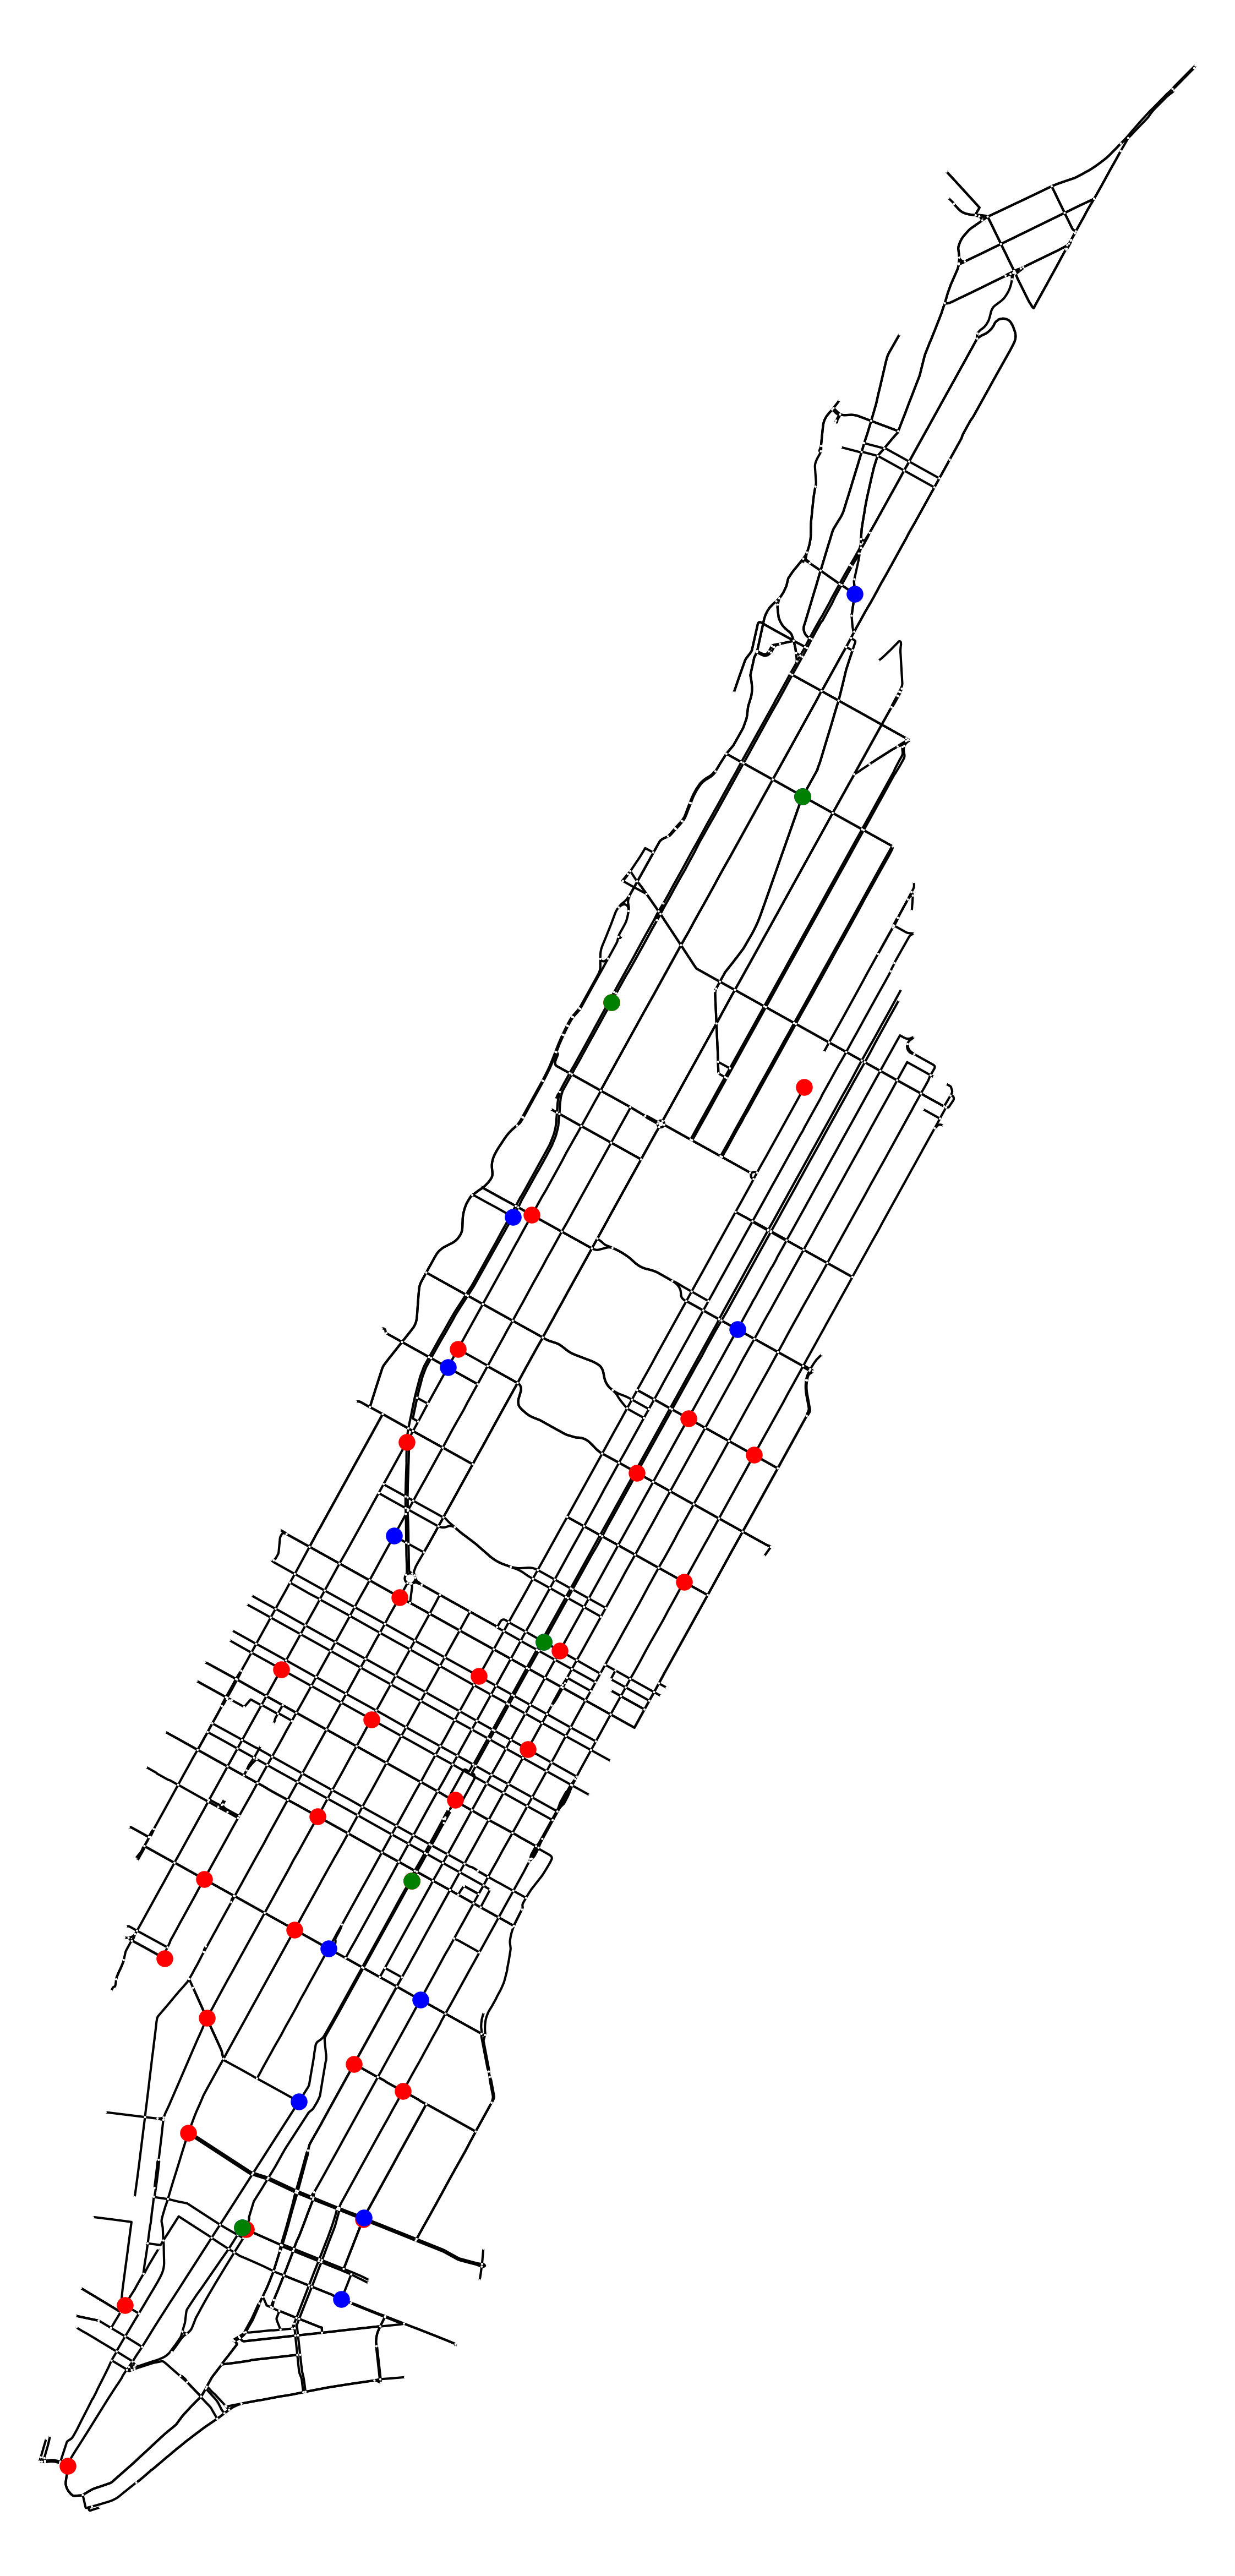
\includegraphics[width=\textwidth]{assets/img/07_graph_based/new_york_simplified_info.png}
		\caption{}
		\label{fig:nyc_simplified_info}
	\end{subfigure}
	\begin{subfigure}[b]{0.32\textwidth}
		\centering
		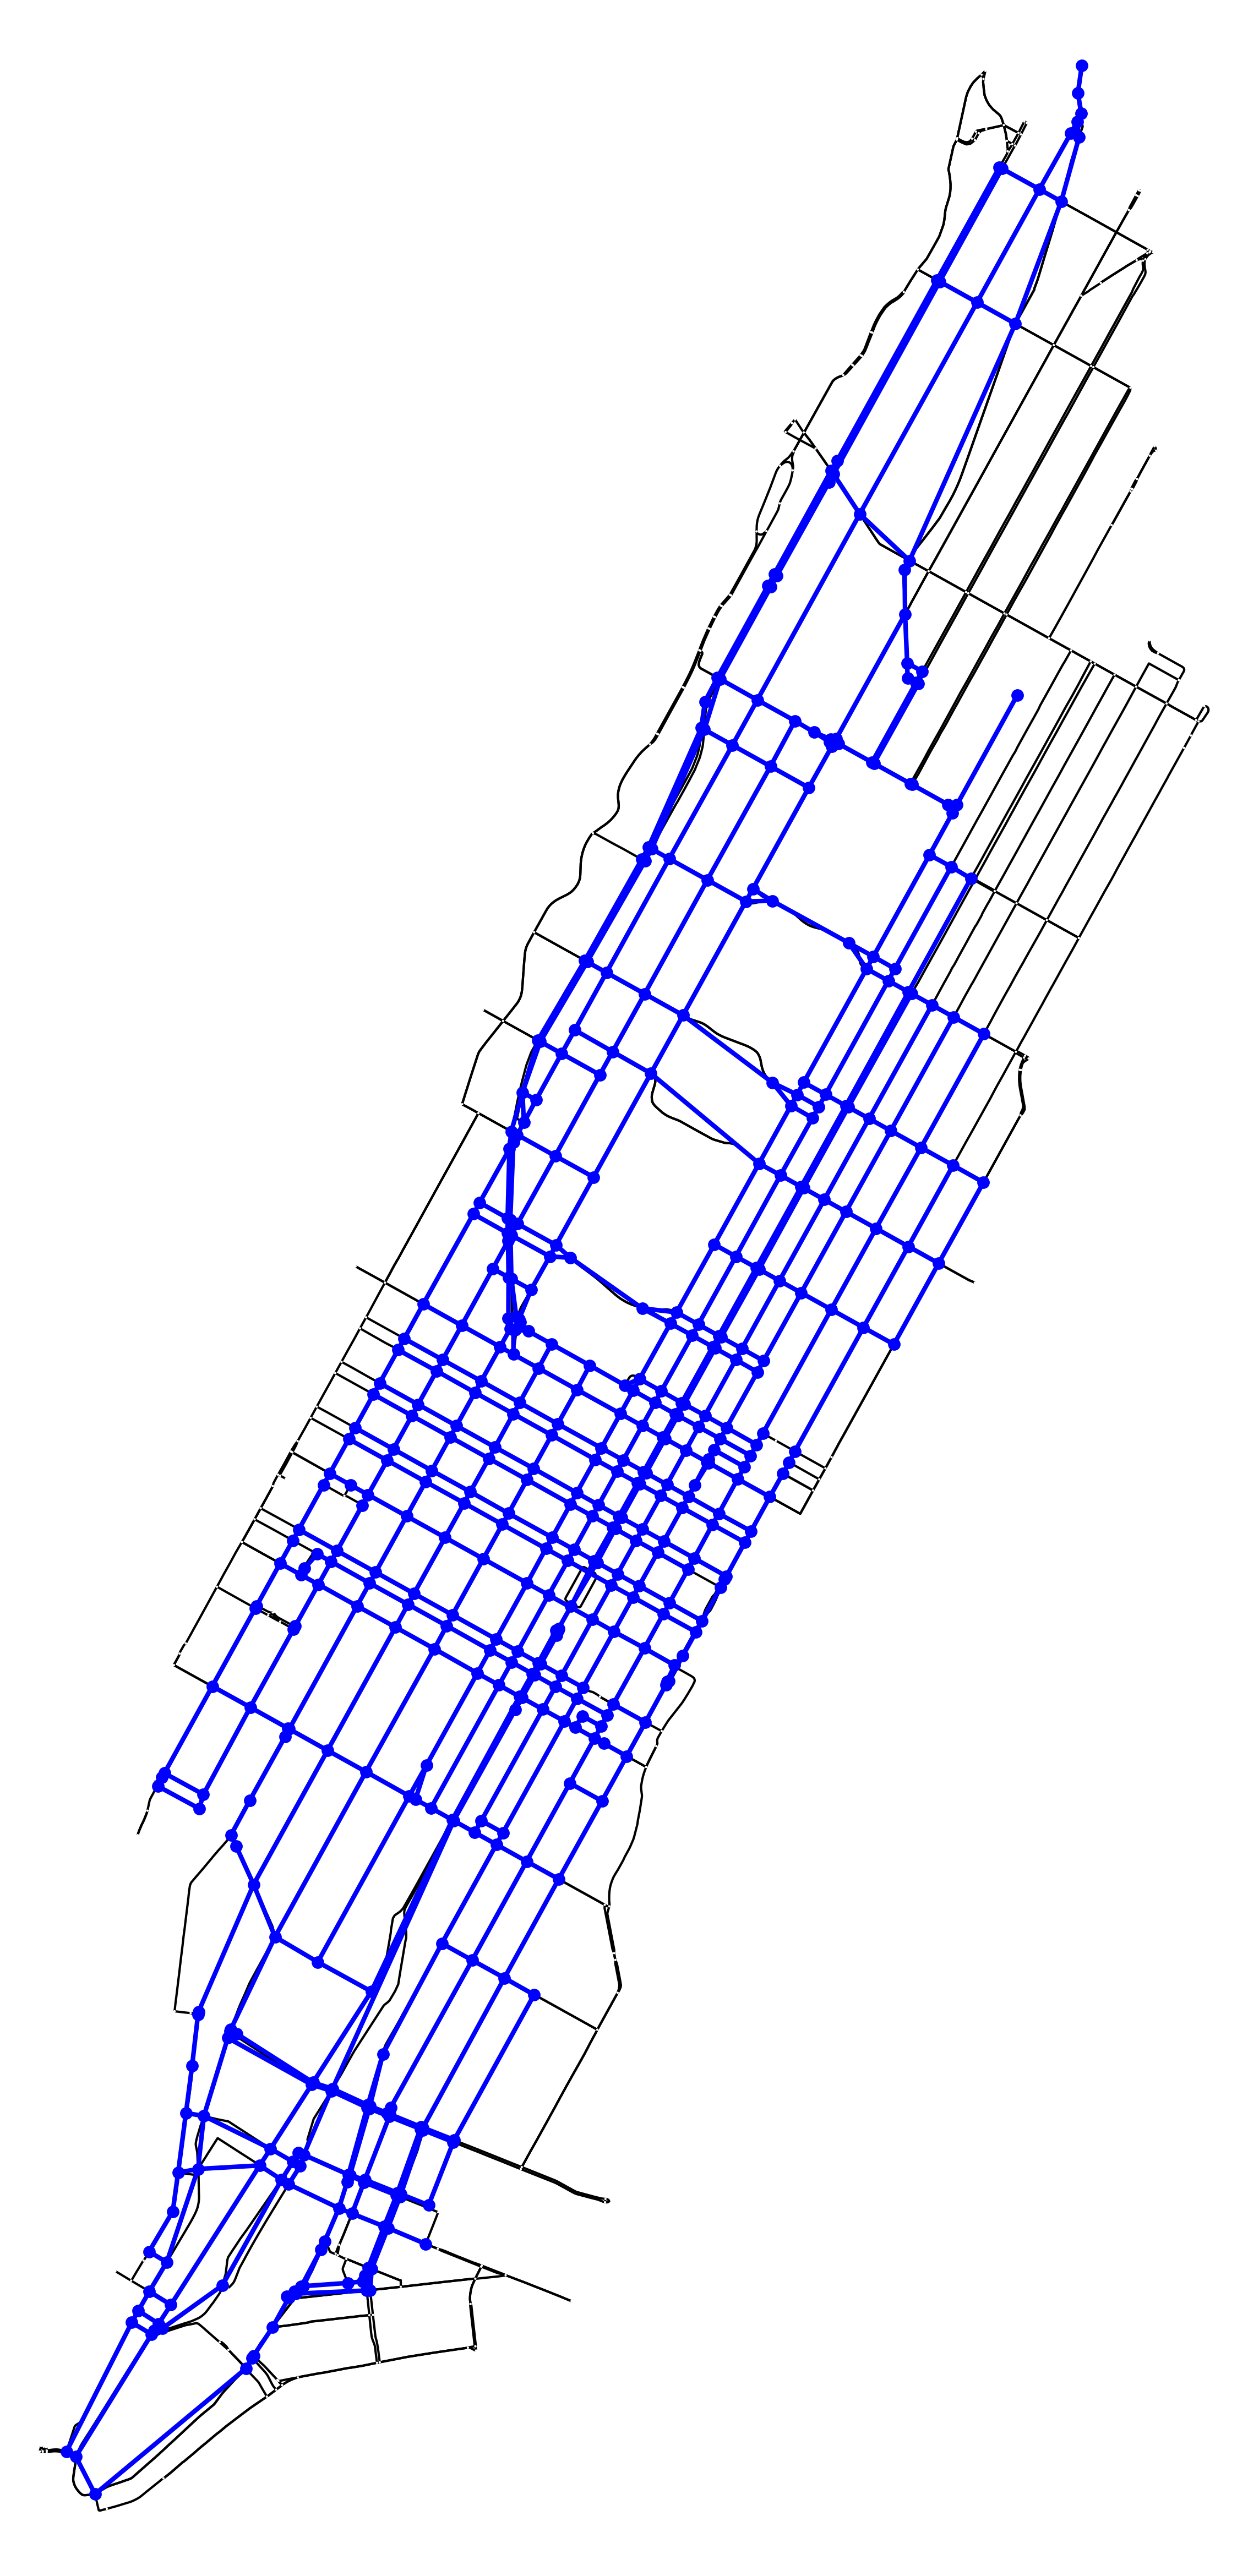
\includegraphics[width=\textwidth]{assets/img/07_graph_based/new_york_simplified_roads.png}
		\caption{}
		\label{fig:nyc_simplified_roads}
	\end{subfigure}
	
	\caption[Manhattan's Road Network Representation]{Manhattan's Road Network Representation. In \subfigref{fig:nyc_rn_info}, red points are used to indicate pick-up stations, while blue delineates drop-off points and green is used to pin-point the fictitious depots. These are obtained by the historical data. Furthermore, pick-up points can also be used as drop-off, and viceversa. \subfigref{fig:nyc_simplified_info} shows the semplified road network consisitnf of only the most important streets. Finally, \subfigref{fig:nyc_simplified_roads} shows the final version of the road network after the application of the minimum spanning tree algorithm.  }
	\label{fig:nyc_rn}
\end{figure}
The main purpose of this use case is to demonstrate the applicability of the model in the real world and the feasibility of the solutions presented in \secref{sec:prob_form}. This use case is based on real-world data extracted from taxi rides in manhattan in 2016 (\cite{Donovan2014}). \\
The data has been prepared in the following way. Since the data retrieved is based on the whole New York City, in order to decrease the complexity, some filters have been applied to only target the Manhattan area. More specifically, the pick-up and drop-off points which were outside of Manhattan have been filtered out. Subsequentially, these pick-up and drop-off points have been clustered in 40 locations. Finally, these locations have been mapped to the real Manhattan road network and the shortest path between five neighbours nodes has been traced in order to create a simplified road network, which can be seen in \figref{fig:nyc_rn}. \\
As a consequence, the complexity of Manhattan's road network has been significantly reduced. Within the context of this project, and specifically in this section, this simplification is deemed acceptable since only proof of concepts are being considered. Furthermore, employing a more intricate representation of the road network would not significantly enhance the objectives at hand. This streamlined approach not only facilitates clearer demonstration of concepts but also expedites the analysis process, enabling a more focused examination of essential elements. Thus, for the current scope of this work, the simplified representation remains suitable and pragmatic.
According to the discussion in \secref{sec:rebal}, the region has been divided in multiple areas as well. This can be observed in \figref{fig:nyc_rn_info}. Although the division in areas it's not explicitely stated, five green-highlited nodes can be observed. These nodes represent depots and have been created to fulfill the same purpose of \secref{sec:rebal}.  In order to improve the performance of the simulation, the road network has been simplified by considering only the most important streets in Manhattan, as shown in \figref{fig:nyc_simplified_info} and \figref{fig:nyc_simplified_roads}. This approach optimizes resources while still providing valuable insights into the model performance. \figref{fig:nyc_simplified_roads} specifically has been obtained by first calculating the shortest path, in terms of distance, of the points highligthed in \figref{fig:nyc_rn_info}. Furthermore, the Minimum Spanning Tree (MST) algoritm (\cite{networkx2021}). The MST is used to calculate the smallest possible connected subtree that spans all the vertices in a given graph. In essence, constructing MST involves iteratively selecting edges with the smallest weight while ensuring that no cycles are formed. This process starts with any arbitrary vertex and gradually expands by adding the lightest edge connected to the existing tree until all vertices are encompassed.\\
While information regarding customer demands are relatively easy to obtain, other data must be crafted or estimated. In particular, details about the constraints outlined in \secref{sec:vc_model} can be challenging to gather as they are often specific to certain scenarios or dependent on external factors not captured by the model. For instance, determining the threshold in the congestion model is complex, especially considering it could easily reach thousands in a densely populated city like NYC. Likewise, the time windows of a request is also very specific to the application. For the rest of this work, this information will be derived from the available data and created, if required. For example, the traveling time for each link $T^a_{u,v}$ can be derived with the assumption of a constant speed. Trivially, since the distance is known, the travelling time can be calculated as follows: \\
\begin{equation}
	T^a_{u,v} = \dfrac{d_{u,v} }{l_{u,v}}
\end{equation}
where $l_{u,v}$ is the speed limit of the link $\langle u,v\rangle$. \\
Although data on customer mobility is readily accessible, obtaining precise information on goods delivery poses a challenge. This includes details on the specific category of goods being transported and the exact dropoff locations. Multiple might be the reasons for it, such as privacy, commercial sensitivity or due to the highly heterougenous nature of this field. Nevertheless, a potential approach to glean insights into goods delivery could involve leveraging publicly accessible datasets such as the GetFood Historical Data (\cite{getfoodnyc}). Amid the COVID-19 pandemic, initiatives like GetFoodNYC have been instrumental in facilitating emergency home food delivery for residents unable to access food through conventional means. Although the data provided does not contain delivery location, this can be simulated by picking a random location within the road network and the quantity can be estimated by the available data.\\
The simulations have been carried out using the CBC (\cite{schumacher2022rcbc}) and Gurabi (\cite{gurobi}) solvers used in combination with PuLP (\cite{dunning2011pulp}) on a 2018 Intel i7 MacbookPro. 

\begin{figure}[t]
	\centering
		\begin{subfigure}[b]{0.5\textwidth}
		\centering
		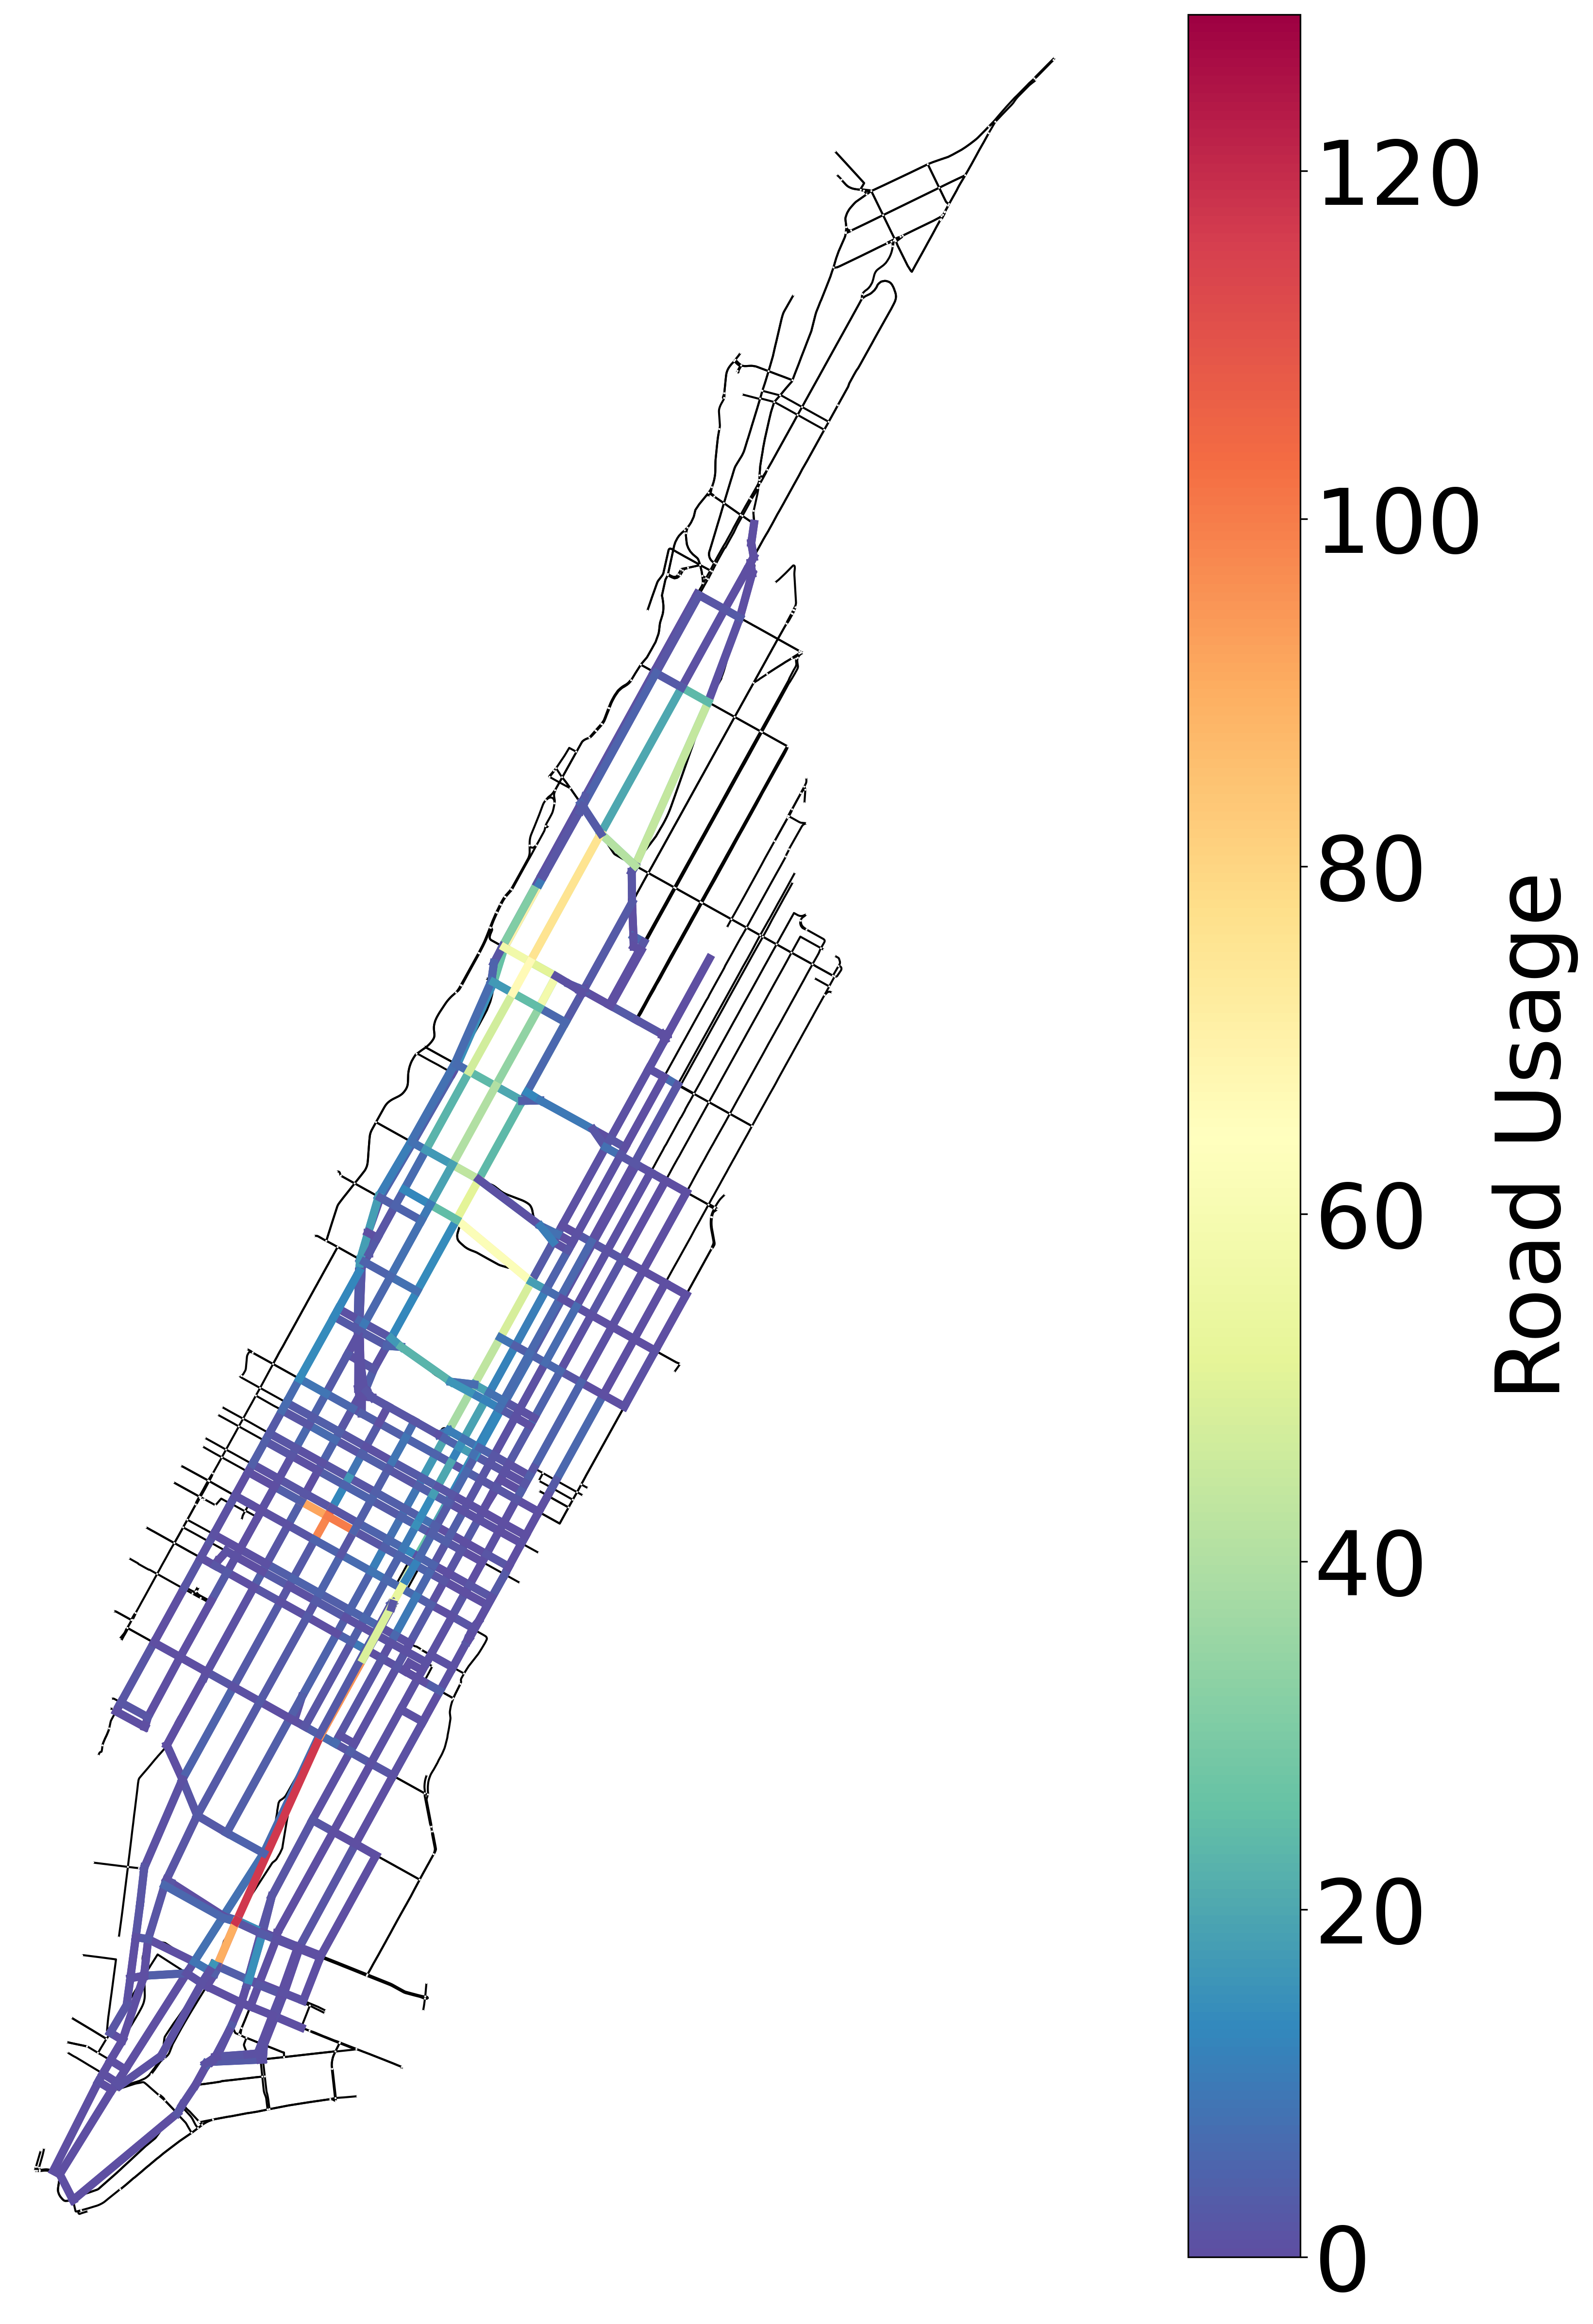
\includegraphics[width=\textwidth]{assets/img/07_graph_based/nyc_road_usage.png}
		\caption{}
		\label{fig:nyc_road_usage}
	\end{subfigure}
	\hfill
	\begin{subfigure}[b]{0.45\textwidth}
		\centering
		\begin{tikzpicture}
			\begin{axis}[
				xbar,
				ytick=data,
				ytick={1,10,20,30,40},
				ylabel={Vehicle Id},
				xlabel={Charge (\%)},
				bar width=3pt,
				%yticklabel pos=right,
				xmajorgrids=true,
				xticklabel pos=right,xlabel near ticks,
				grid style=dashed,
				yticklabel pos=right, ylabel near ticks,
				minor y tick num=9,
				ytick style={draw=none},
				]
				\addplot coordinates {
					(96.40179272992049,1)
					(94.89649535146043,2)
					(94.33360135023348,3)
					(90.41910053961556,4)
					(89.23245976372155,5)
					(89.1620959397407,6)
					(91.9661039386619,7)
					(88.52102127563072,8)
					(88.39057851690268,9)
					(87.83262408504747,10)
					(85.16152711790919,11)
					(85.78292039341194,12)
					(86.82803084732097,13)
					(86.37232542782782,14)
					(84.66212090585896,15)
					(86.8216077893955,16)
					(86.93174672079786,17)
					(86.0718514488063,18)
					(82.05741551782936,19)
					(84.54190526183835,20)
					(86.9579883628448,21)
					(88.95263072465707,22)
					(88.95632720433568,23)
					(89.72727505023411,24)
					(87.89324287497183,25)
					(89.72205766995334,26)
					(91.06841139591609,27)
					(92.99588049178772,28)
					(93.83580167946283,29)
					(94.00346732723801,30)
					(93.69881531144985,31)
					(90.46223889616006,32)
					(90.71528686407433,33)
					(87.23929616120468,34)
					(87.29955925950475,35)
					(88.8375639554714,36)
					(87.85363969943707,37)
					(90.94051744267162,38)
					(92.92330301589077,39)
					(95.62956196834227,40)
				};
			\end{axis}
		\end{tikzpicture}
		\caption{ }
		\label{fig:my_bar_plot_horizontal}
	\end{subfigure}
	\caption[Overview of System's Performance without Congestions]{ 
	\subfigref{fig:nyc_road_usage} illustrates the utilization of the entire road network during the whole shift. Road usage is determined by aggregating the total number of vehicles traversing each road segment throughout the shift duration.  \subfigref{fig:my_bar_plot_horizontal} displays the average vehicle charge during the shifts.
	}
	\label{fig:nyc_analysis_no_congestions}
\end{figure}
\subsection{Road Usage Without  Congestions}
An overview of the system performance can be observed in \figref{fig:nyc_analysis_no_congestions}. 

\begin{itemize}
	\item Analyse the following metrics
	\begin{itemize}
		\item Road usage
		\item Vehicle Charge at the end
		\item Vehicle distribution at the end of the shift
		\item Vehicles travel time
	\end{itemize}
	
	
\end{itemize}


%\section{TO-DO}
%\begin{itemize}
%	\item Make the battery model in terms of the links. The time is, basically, the velocity of that link over the distance.
%	\item The time must be adapted according to the link travelling time. I.e., each request has a time window. The time from the inbound link must be within the time window.
%	\item Create a simulation using some fake data
%\end{itemize}
%\begin{itemize}
%	\item maybe use  a kalman filter to estimate requests per time
%\end{itemize}

\chapter{Model Predictive Control of AToD}\label{ch:mpc}
\section{Linear-Discrete Time Model}\label{sec:linear_discrete_time_model}
The model derived in this section is partially inspired from \cite{zhang2016}. \\
Consider a transportation network be composed of $|\mathcal{V}|$ stations scattered around a space $\Omega$ and $|\mathcal{A}|$ multi-occupancy, goods-carrying vehicles working within the same space $\Omega$. Within this context, customers are assumed to requests rides only from the abovementioned stations. Similarly, goods can be carried out only from one station to another. With this assumption, stations and customers can be considered synonims within this section. \\
Similarly to the model described in \chapref{sec:vc_model}, other than carrying goods or people, vehicle are expected to \textit{(i)} serve clients from one station to another and \textit{(ii)} reach locations in $\Omega$ in order to avoid system imbalance. \\
Let $d_{ij} \in \mathcal{R}_{\ge0}$ be the total lenght of a road \(\langle i,j\rangle\). Let $v^a_{ij}(t) \in \{0,1\}$ indicate whether a transporting vehicle $a \in \mathcal{A}$ is moving from station $i$ to station $j$ ($v^a_{ij}(t) = 1$) and, likewise, $w^{a}_{ij}\in \{0,1\} $ whether an empty vehicle is moving from $i$ to $j$ ($w^{a}_{ij}(t)= 1$). Let $V_{ij}(t) = \sum_{a \in \mathcal{A}} v^{a}_{ij}(t) +w^{a}_{ij}(t)$ being the total number of vehicles currently circulating on the street $\langle i,j\rangle$, it follows that $V_{ij}(t) \in \mathbb{N}_+$. \\
When a vehicle is in transit, it is essential to monitor the anticipated duration until it reaches its destination. In order to do so, let's assume the road $\langle i,j\rangle$ to have a speed limit $l_{i,j}$. Accordingly, since the system is dealing with fully autonomous vehicles, in a typical driving scenario, one can safely assume this to be the cruising speed as well. In other words, one can assume the vehicles to be driving with a speed $l_{i,j}$ over $\langle i,j\rangle$ in normal road conditions.  Motivated by safety concerns, the cruising speed cannot be consistently maintained at \(l_{i,j}\) due to various factors. These factors may include road conditions, weather conditions, traffic density, or any unforeseen circumstances. Therefore, the actual cruising speed during the journey over road \(\langle i,j\rangle\) may vary based on these dynamic elements, ensuring that the autonomous vehicles can adapt to changing conditions and prioritize safety over a fixed cruising speed. One factor which is directly controllable is the traffic density. Therefore, taking inspiration from the BPR model (\figref{fig:bpr_models_approx}), we can approximate the cruising speed according to the amount of vehicles on the road. More specifically, we can modify \equaref{eq:model_bpr_approximation} to reflect this condition, and therfore rewriting it as \\
\begin{equation}
	\begin{aligned}	
		s_{ij}(V_{ij}) &= \begin{cases}
			l_{ij} \quad\quad &\text{if } V_{ij}\in[0,V_{ij}^{th}]\\ 
			l_{ij} - b\cdot(V_{ij} - V_{ij}^{th}) \quad\quad &\text{if }V_{ij}\in[V_{ij}^{th}, V_{ij}^{max}]\\ 
			0\quad\quad &\text{if }V_{ij} \ge V_{ij}^{max}\\ 
		\end{cases}\\
		\text{with } b  &=  \dfrac{l_{ij}}{ V_{ij}^{th} -  V_{ij}^{max}}
\end{aligned}
	\label{eq:model_bpr_approximation2}
\end{equation}
An example can be seen in \figref{fig:speed_model}. The last case, i.e. when $V_{ij} \ge V_{ij}^{max}$, is inspired from the congestion model used in \secref{sec:vc_model} and in this case is modeling stale mate traffic. Intuitively, if too many cars are on the road, these will not be able to circulate with a high speed and eventually stop-and-go traffic will be created. \\
From the definition, it follows that $s_{if}$ is defined as $s_{ij}: \mathbb{N}_{+} \rightarrow \mathbb{R}_{\ge 0}$.

\begin{figure}[t]
	\centering
	\begin{tikzpicture}
		\begin{axis}[
			xlabel={$V_{ij}$},
			ylabel={$s_{ij} (km/h)$},
			domain=0:250, % adjust the domain based on your preference
			samples=40,
			grid=both,
			axis x line=middle,
			%ymin=-1, % Set the minimum y-axis value
			%ymax=1.4, % Set the maximum y-axis value
			axis on top,
			legend pos=north east
			]
			% Piecewise function
			\addplot[blue, thick, domain=0:100] {60};
			\addplot[blue, thick, domain=100:150] {60 - 1.2*(x-100)};
			\addplot[blue, thick, domain=150:200] {0};
			%\addlegendentry{B}
		\end{axis}
	\end{tikzpicture}
	\caption[Cruising speed in function of traffic density]{Cruising speed in function of traffic density. In this example, $l_{ij} = 60 km/h,V_{ij}^{th} = 100$,$V_{ij}^{max} = 150$.  }
	\label{fig:speed_model}
\end{figure}
This allows to effectively track the position of the vehicle in terms of time as well. However, the position should be tracked only if the vehicle is currently driving on the street. 
Therefore, position of the vehicle $a$ over $\langle i,j\rangle$ is propagated using \equaref{eq:position_propagation}. 
\begin{equation}
	x^a_{ij}(t+\delta) =\begin{cases}
		 x^a_{ij}(t) + s_{ij}(V_{ij}(t))\cdot\delta & \text{if } v^a_{ij}(t) + w^a_{ij}(t)= 1 \\
		 
		 0& \text{if } v^a_{ij}(t) + w^a_{ij}(t)= 0\\
		 0& \text{if }i=j \\
		 %0 & \text{otherwise}
	\end{cases}
	 \label{eq:position_propagation}
\end{equation}
As mentioned above, \equaref{eq:position_propagation} tracks the position of a moving vehicle, i.e. takes care of the state of moving vehicles. In addition to this, the model also needs to track the number of vehicles currently stationed in $i$. This is achieved by introducing an additional variable $f^a_i(t)$, which indicates whether a vehicle arrived at a station $i$. It is defined as following.
\begin{equation}
	f^a_{i}(t) =\begin{cases}
		1 & \text{if }x^a_{ji}(t)= d_{ji}\\
		0 & \text{otherwise}
	\end{cases}
	\label{eq:station_propagation}
\end{equation}
This is propagated with the help of the indicator function. 
\begin{equation}
	f^a_i(t+1) =f^a_i(t) + 1_{d_{ji} = x^a_{ji}(t)} - \sum_{j\in\mathcal{V}}(v_{ij}^a + w_{ij}^a) %1_{d_{ji} \neq x^a_{ji}(t)}
	\label{eq:stationed_propagation_ind}
\end{equation}
\equaref{eq:stationed_propagation_ind} also ensures that a vehicle performs an action on the road $\langle i,j\rangle$ only when stationed at $i$.\\
%\begin{equation}
%	f^a_i(t+1) = f^a_i(t) +1_{d_{ji} = x^a_{ji}(t)} - \sum_{j \in \mathcal{N}}( v^a_{ij} + w^a_{ij})
%	\label{eq:stationed_propagation}
%\end{equation}
The function $1_x$ is commonly known as the indicator function, denoting a Boolean variable x that can take values {true, false}. Specifically, $1_x$ is defined as follows:
\begin{equation}
	1_x = \begin{cases}
		1 & \text{if } x \text{ is true} \\
		0 & \text{if } x \text{ is false}
	\end{cases}
\end{equation}
In other words, $1_x$ equals 1 when x is true and equals 0 when x is false, making it a convenient way to express the truth value of the variable x in mathematical notation.\\
Crucially, the vehicles can not perform the aforementioned actions, i.e. waiting, routing and rebalancing, at the same time and this must be insured. Furthermore, the vehicles can not perform the actions on multiple stations or roads. Therefore, the following constraint is necessary. \\
\begin{equation}
	\sum_{i \in \mathcal{V}}(f^a_{i}(t+1)+\sum_{j \in \mathcal{V}}v^a_{ij}(t) + \sum_{j \in \mathcal{V}}w^a_{ij}(t)) = 1\label{eq:no_3_actions}
\end{equation}
This also implies that, if a vehicle is stationed at a station $i$, it can not have a position anywhere else. 
\begin{equation}
	%0<\sum_{i \in \mathcal{V}}(f^a_{i}(t)+\sum_{j \in \mathcal{V}}\dfrac{x^a_{ij}(t)}{d_{ij}}) \leq1 \label{eq:position_station}
	%d_{ji}
	\sum_{i \in \mathcal{V}}(f^a_{i}(t)+1_{ x^a_{ji}(t)\neq 0}) =1 \label{eq:position_station}
\end{equation}
In other words, if I vehicle is travelling through an edge $\langle ji\rangle$, it can only be stationed at $i$ if it finished travelling. \\
While it is on the one hand interesting to know which station is currently hosting which vehicle, it is more important to know the amount of vehicles currently circulating in the system. This can be achieved by flipping the idea and therefore calculating how many vehicles out of the total number is currently not stationed. 
\begin{equation}
	F(t) = |\mathcal{A}| - \sum_{i \in\mathcal{N}}\sum_{a \in\mathcal{A}}f^a_{i}
\end{equation}
Furthermore, one can also calculate the required time $T_{ij}(t)$ based on the speed approximation, as shown in \equaref{eq:required_time}. 
\begin{equation}
	T_{ij}^a(t) = \begin{cases}
		\dfrac{d_{ij} - x^a_{ij}(t)}{s_{ij}(V_{ij}(t))} &\quad \text{if } x_{ij}^a(t) > 0\\
		&\\
		0 &\quad\text{otherwise }
	\end{cases}
	\label{eq:required_time} 
\end{equation}

Denoted by $p_{ij}(t)$ and $g_{ij}(t)$ are the transportation and goods delivery requests respectively starting from station $i$ and headed to $j$. Let $o^p_{ij}(t)$ and $o^g_{ij}(t)$ denoting the number of outstanding requests from $i$ to $j$ for people or goods, respectively, one can describe its propagation as follows:

\begin{equation}
	\begin{aligned}
		o^p_{ij}(t+1) =& o^p_{ij}(t) + p_{ij}(t) - \sum_{a \in \mathcal{A}} P_a\cdot v^a_{ij}(t)\\
			o^g_{ij}(t+1) =& o^g_{ij}(t) + g_{ij}(t) - \sum_{a \in \mathcal{A}} G_a \cdot v^a_{ij}(t)\\
	\end{aligned}
	\label{eq:demand_time}
\end{equation}
%Furthermore, when a vehicle leaves, it can only leave 
It follows then that vehicles can not transport more than what requested, i.e.:
\begin{equation}
	\begin{aligned}
	\sum_{a \in \mathcal{A}}  P_a\cdot v^a_{ij}(t) &\leq o^p_{ij}(t) + p_{ij}(t) \\
	\sum_{a \in \mathcal{A}} G_a \cdot v^a_{ij}(t) &\leq o^g_{ij}(t) + g_{ij}(t)
	\end{aligned}
	 \label{eq:no_more_than_request}
\end{equation}


At this point, the definition of the control and the state of the system is complete. More specifically, the state of the system is described by the number outstanding requests $o_{ij}(t)$, the position of each moving vehicle $x_{ij}(t)$ and the position of each idle vehicle $f^a_{i}(t)$. Let the vector x(t) be the column vector column vector created by reshaping and concatenating $o_{ij}(t)$, $x_{ij}(t)$, $T_{ij}^a(t)$ and $f^a_{i}(t)$, the set of feasible states $\mathcal{X}$ is defined as follows. 

\begin{equation}
	\mathcal{X} := \left\{
	\begin{aligned}
		& o^p_{ij} \in (\mathbb{N}_+)^{|\mathcal{V}|},o^p_{ii} = 0, o^g_{ij} \in (\mathbb{N}_+)^{|\mathcal{V}|},o^g_{ii} = 0   \\
		 x = [o^p_{ij},o^g_{ij}, x_{ij}^a, f^a_{i}, T_{ij}^a]^T \Bigg| &f^a_{i} \in \{0,1\}^{|\mathcal{A}||\mathcal{V}|}, \text{(\ref{eq:position_station})} \\
		&  x_{ij}^a\in (\mathbb{R}_{\ge 0})^{|\mathcal{A}||\mathcal{V}|}, T^a_{ij} \in (\mathbb{R}_{\ge 0})^{|\mathcal{V}|} \\
	\end{aligned}
	\right\}
\end{equation}
%Note that because of  \equaref{eq:position_propagation}, the set of feasible states is time-dependent. 
Similarly, considering the control inputs $v^{a}_{ij}(t)$ and $w^{a}_{ij}(t)$, one can derive the set of feasible control set $\mathcal{U}(t)$ as follows. 
\begin{equation}
	\mathcal{\mathcal{U}}(t) := \left\{
	\begin{aligned}
		&v^a_{ij} \in \{0,1\}^{|\mathcal{A}||\mathcal{V}|}, v^a_{ii} = 0 \\
		u = [v^{a}_{ij}, w^{a}_{ij}]^T \Bigg|&w^a_{ij} \in \{0,1\}^{|\mathcal{A}||\mathcal{V}|},w^a_{ii} = 0 \\ 
		&\text{(\ref{eq:no_3_actions}),(\ref{eq:no_more_than_request})
		} \\
	\end{aligned}
	\right\}
\end{equation}
Since (\ref{eq:no_3_actions})-(\ref{eq:no_more_than_request}) depend on time, $\mathcal{U}(t)$ is also time-dependent. \\
Thanks to these formulations, the system can be written as a linear time-dependent system of the form
\begin{equation}
	x(t+1) = Ax(t) + Bu(t)\label{eq:normal_system}
\end{equation}
where $x(t) \in \mathcal{X}$, $u(t) \in \mathcal{U}(t)$ and $A$ and $B$ are the matrix associated to the coefficients of (\ref{eq:position_propagation}), (\ref{eq:stationed_propagation_ind}) and (\ref{eq:demand_time}). \\


\subsection{Model Evaluation}
Some comments are in order. Requests are treated considering customers and goods as single entities. More specifically, if a group consisting of three customers reach a station, this is treated as three individual requests, therefore $p_{ij}(t) = 3$. While this simplifies the model description and reflects the requirements for goods delivery, it would create an inconvenient scenario for traveling customers. As a matter of fact, it is not hard to envision situations where a group of travelers would like to travel together. However, it is out of the scope of this work to treat this scenario. One might also argue that this simplification effectively treats the model as if vehicles where single-occupancy and it is true in terms of intuition, this addition allows to reduce the number of variables by a constant factor, i.e. the sum of all vehicles' capacity. \\
The system described in \equaref{eq:normal_system} implicitely assumes the customer arrival to be known a priori. In order words, this is not treated as noise, but rather as a known quantity. 
\begin{equation}
	x(t+1) = Ax(t) + Bu(t) + w(t)\label{eq:disturbed_mpc_formulation}
\end{equation}
where $x(t) \in \mathcal{X}$, $u(t) \in \mathcal{U}(t)$, $w(t) = [p_{ij}(t)\quad g_{ij}(t)\quad0\quad0 \quad0]^T$ and $A$ and $B$ are the matrix associated to the coefficients of (\ref{eq:position_propagation}), (\ref{eq:station_propagation}) and (\ref{eq:demand_time}). \\
\equaref{eq:disturbed_mpc_formulation} treats customer arrival as noise, or disturbance, which makes reasoning on the system considerably harder. Several techniques (\cite{Campo1987RobustMP}, \cite{LANGSON2004125}) have been proposed to deal with this type of MPC systems, i.e. Robust MPC.  Alternatively, some work propose solutions to estimate this quantity using Deep Learning techniques (\cite{9202791}, \cite{8569427}).
However, the analysis of those techniques and their performance in this scenario is out of the scope of this work.
Similarly to \secref{sec:vc_model}, the model must take into account that stations do not have unlimited amoun t of parking spots. As a consequence, the number of vehicles stationed must be limited accordingly and this is achieved as follows. 
\begin{equation}
	\sum_{a \in \mathcal{A}}f^a_i(t) \leq C_i
	\label{eq:parking_limit}
\end{equation}
where $C_i$ indicates the number of parking spots available at $i$. \\
This is a crucial 

\section{Problem Formulation}
The MPC for the AToD problem is formulated as follows. \\
Given $x(t) \in \mathcal{X}$, determine the controls $u(t), \dots, u(t+N)$ according to the following optimization problem.
\begin{equation}
	\begin{aligned}
		\underset{\substack{u(t), \dots, u(t+N)}}{\text{\textbf{min}}} \quad & J_f(x(N))+\sum_{t=0}^{N-1}I(x(t)) \\
		\text{\textbf{s.t.}} \quad & x(t+1) = Ax(t) + Bu(t)  \\
		& x(t) \in \mathcal{X}, \ u(t)\in \mathcal{U} \\
		%& k = t, \dots, t+N\\
		&x(N) \in \mathcal{X}_f\\
	\end{aligned}
	\label{eq:mpc_atod}
\end{equation}
where $J_f(x(t+N))$ is the terminal cost function and $\mathcal{X}_f$ is the terminal set. \\
As the main goal is to prove the stability of (\ref{eq:mpc_atod}), a proper definition of those will facilitate this objective. The strategy used to prove stability is the one described in \secref{sec:stable_mpc_systems}. For this purpose, the terminal set is required to be defined around an equilibrium point $x_*$. A good canidate for the equilibrium point in such systems can be found by observing that the system remains at a equilibrium whenever no more requests arrive and the are no more outstanding requests within the system. In other words, when 
\begin{align*}
	p_{ij}(t) &=0 \\
	g_{ij}(t) &=0\quad\quad \forall i,j\in\mathcal{V}\\
	o^p_{ij}(t) &=0\\
	o^g_{ij}(t) &=0\\
\end{align*}
By \equaref{eq:demand_time}, this implies that, eventually, no more vehicles will transport goods or people anymore. Furthermore, one can also conclude that vehicles will also stop rebalancing themselves. Therefore, $o_{ij}, x_{ij}^a$ and $T_{ij}^a$ all assume value zero. However, there is no way of knowing exactly where vehicles are going to be stationed. Upon inspection, however, one can canclude that vehicles must be stationed somewhere, since they are not driving. In other words, $f^a_{i}$ could assume any value in $\{0,1\}^{|\mathcal{A}||\mathcal{V}|} $ except $ \{0\}^{|\mathcal{A}||\mathcal{V}|}$. Furthermore, at equilibrium, all the vehicles are stationed. That means, the set of possible values for  $f^a_{i}$ is further limited accordingly. To define this set, let's consider a function $n : \mathcal{D}_{f^a_{ij}} \rightarrow N$, where $\mathcal{D}'_{f^a_{ij}}  = \{0,1\}^{|\mathcal{A}||\mathcal{V}|} \setminus \{0\}^{|\mathcal{A}||\mathcal{V}|}$, which sums the number of 1s in the set. With this addition, we can fully define the set of values of $f^a_{i}$  at equilibrium. 
\begin{equation}
\mathcal{D}_{f^a_{ij}} := 	\left\{
	x   \quad | \quad x \in \{0,1\}^{|\mathcal{A}||\mathcal{V}|},  n(x) = |\mathcal{A}|
	\right\}\label{eq:set_of_fs}
\end{equation}
%($\binom{|\mathcal{A}||\mathcal{V}|}{|\mathcal{A}|}$)
While the set is indeed smaller, it is still quite hard to exactly pin-point a specific equilibrium point, as already mentioned above. The difficulty arises because, out of all the elements in (\ref{eq:set_of_fs}), one can not directly identify the one which describes the system fully without knowing how the system progressed in time. However, one can conclude that the equilibrium points are all elements of the set described in \equaref{eq:final_eq}. 
\begin{equation}
	\mathcal{E} := \left\{
	\begin{aligned}
		& o^p_{ij} \in \{0\}^{|\mathcal{V}||\mathcal{A}|} , o^g_{ij} \in \{0\}^{|\mathcal{V}||\mathcal{A}|}  \\
		e = [o^p_{ij},o^g_{ij}, x_{ij}^a, f^a_{i}, T_{ij}^a]^T \Bigg| &f^a_{i} \in \mathcal{D}_{f^a_{ij}}   \\
		&  x_{ij}^a\in\{0\}^{|\mathcal{V}||\mathcal{A}|} , T^a_{ij}\in \{0\}^{|\mathcal{V}||\mathcal{A}|} \\
		%&  x_{ij}^a\in (\mathbb{R}_{\ge 0})^{|\mathcal{A}||\mathcal{V}|}, T^a_{ij} \in (\mathbb{R}_{\ge 0})^{|\mathcal{V}|} \\
	\end{aligned}
	\right\}\label{eq:final_eq}
\end{equation}\\
While this could be considered as a candidate for the terminal set $\mathcal{X}_f$, it turns out to be too restrictive. This is due to the fact that it would require all vehicles to be stationed and, therefore, not moving. Some of the conditions, however, can be relaxed by considering some implicit assumptions made during the development of the model. Mainly, vehicles are assumed to be perfect and to never break, therefore, one can consider a request to be satisfied the moment it has been picked up. As a result, while the number of requests is still zero, the conditions for $x_{ij}^a$, $f_{i}^a$ and $T_{ij}^a$ can be relaxed. 
\begin{equation}
	\mathcal{X}_f := \left\{
	\begin{aligned}
		& o^p_{ij} \in \{0\}^{|\mathcal{V}||\mathcal{A}|} , o^g_{ij} \in \{0\}^{|\mathcal{V}||\mathcal{A}|}  \\
		x_f = [o^p_{ij},o^g_{ij}, x_{ij}^a, f^a_{i}, T_{ij}^a]^T \Bigg| &f^a_{i} \in \{0,1\}^{|\mathcal{V}||\mathcal{A}|}  , \text{(\ref{eq:position_station})}   \\
		%&  x_{ij}^a\in\{0\}^{|\mathcal{V}||\mathcal{A}|} , T^a_{ij}\in \{0\}^{|\mathcal{V}||\mathcal{A}|} \\
		&  x_{ij}^a\in (\mathbb{R}_{\ge 0})^{|\mathcal{A}||\mathcal{V}|}, T^a_{ij} \in (\mathbb{R}_{\ge 0})^{|\mathcal{V}|} \\
	\end{aligned}
	\right\}\label{eq:final_x_f}
\end{equation}\\
By definition, therefore, $\mathcal{E} \subset \mathcal{X}_f \subset \mathcal{X}$. \\
In addition, thanks to this definition, another desiderable conditions apply. Since $ x_{ij}^a\in (\mathbb{R}_{\ge 0})^{|\mathcal{A}||\mathcal{V}|}$ and $T^a_{ij} \in (\mathbb{R}_{\ge 0})^{|\mathcal{V}|}$, empty vehicles can also be navigating, which allows rebalancing, too. Moreover, since vehicles are not required to be stationed and the minimum requirement for a request to be satisfied is to be picked up, as long as the capacity of the vehicle stationed in $i$ is enough to cover the request, than the number of outstanding requests is still zero. 
\begin{equation}
\begin{aligned}
	\sum_{a \in \mathcal{A}}  P_a\cdot f^a_{i}(t) &\ge p_{ij}(t) \\
	\sum_{a \in \mathcal{A}} G_a \cdot f^a_{i}(t) &\ge  g_{ij}(t) \quad\quad \forall i,j\in\mathcal{V}\\
	o^p_{ij}(t) &=0\\
	o^g_{ij}(t) &=0\\
\end{aligned}
\label{eq:conserved_rela}
\end{equation}
This further relaxation also allows to better reason about the control law $\kappa_f$ required to prove stability of the controller. The two main requirements are (i) $\kappa_f \in \mathcal{U}$ and (ii) the set $\mathcal{X}_f$ remains feasible, since they are among the main assumption for the controller stability (\secref{sec:stable_mpc_systems}). Furthermore, 
at each time, it is required that the capacity of the vehicle leaving a station is equal to the new demand, as the number of outstanding requests is zero. 
\begin{equation}
	\begin{aligned}
		\sum_{a \in \mathcal{A}}  P_a\cdot v^a_{ij}(t) &=   o^p_{ij}(t) \\
		\sum_{a \in \mathcal{A}} G_a \cdot v^a_{ij}(t) &=   o^g_{ij}(t)
	\end{aligned}
	\label{eq:no_more_than_request_f}
\end{equation}
Vehicles, however, can only leave a station if they are present at that station. On the same note, since there must be enough vehicles at every station to serve the requests, those must be rebalanced in such a way that, once a request arrives, a vehicle is ready to serve it. \\
The control law that must be designed can be seen as a function mapping $\mathcal{X}_f$ to a subset of $\mathcal{U}$, i.e. $\kappa_f:\mathcal{X}_f \rightarrow\mathcal{U}_{\kappa_f} \subseteq \mathcal{U}$. This function must express then need to ''conserve'' the relation in \equaref{eq:conserved_rela}, which has the by product of also satisfying \equaref{eq:no_more_than_request}.\\
 Furthermore, as a vehicle leaves a station, another vehicle must take its place. Therefore, the follow relation must also hold. 
 \begin{equation}
 	\begin{aligned}
 		P_a\cdot v^a_{ij} &\leq \sum_{j \in\mathcal{V}} \sum_{a'\in \mathcal{A} \setminus \{a\}}P_{a'}\cdot	w^{a'}_{ji}\\
 		G_a\cdot v^a_{ij} &\leq \sum_{j \in\mathcal{V}} \sum_{a'\in \mathcal{A} \setminus \{a\}}G_{a'}\cdot w^{a'}_{ji}\\
 	\end{aligned}
 	\label{eq:replace_vehicle}
 \end{equation}
\equaref{eq:replace_vehicle} is used to ensure that, if a vehicle leaves a station, it must be replaced by one or more vehicles with at least the same capacity.
\begin{equation}
	\mathcal{\mathcal{U}}_{\kappa_f}(t) := \left\{
	\begin{aligned}
		&v^a_{ij} \in \{0,1\}^{|\mathcal{A}||\mathcal{V}|}, v^a_{ii} = 0 \\
		u = [v^{a}_{ij}, w^{a}_{ij}]^T \Bigg|&w^a_{ij} \in \{0,1\}^{|\mathcal{A}||\mathcal{V}|},w^a_{ii} = 0 \\ 
		&\text{(\ref{eq:no_3_actions}),(\ref{eq:no_more_than_request_f}),(\ref{eq:replace_vehicle})
		} \\
	\end{aligned}
	\right\}
\end{equation}
It is trivial to demonstrate that $\mathcal{\mathcal{U}}_{\kappa_f}(t) \subseteq \mathcal{U}$. By construction \equaref{eq:no_3_actions} and \equaref{eq:no_more_than_request} are satisfied (the latter specifically from \equaref{eq:no_more_than_request_f}). \\
A remark is required. \equaref{eq:no_more_than_request_f} and \equaref{eq:replace_vehicle} indeed allow vehicles to be replaced and, therefore, potentially take care of the requests. However, in addition to the assumption made for \equaref{eq:no_more_than_request_f}, the state of the system will remain in $\mathcal{X}_f$ only as long as the requests are made within a time interval corresponding to the time required to travel  from the furthest station to the starting station. In other words, this is a very particular case of extrogenous requests. Therefore, for the rest of this section, the external arriving requests will be considered as zero, i.e. $o^p_{ij}(t) =  o^g_{ij}(t) = 0$, therefore treating the system as undisturbed.\\
This assumption also allows to derive an appropriate cost function for the system. As indicated in \secref{sec:stable_mpc_systems}, the candidate terminal cost must be a Lyapunov function (see \secref{sec:general_definitions} for more details).  \\
Within the assumptions made, one candidate for the terminal cost function can be found by observing the vehicles that are still driving around the system. \\
Intuitively, one can consider the time that the vehicles will spend on the road. At first glance, according to the definition found in \equaref{eq:required_time}, this would be difficult to prove to be Lyapunov. As a matter of fact, the speed of the vehicles depends on the amount of vehicles on the road, which would mean the function is not guaranteed to strictly decrease. In this situation, however, since we are dealing with an undisturbed system near its equilibrium, new vehicles will not be put it motion. In other words, at time $t$, if there are $\sum_{i \in \mathcal{V}}\sum_{j \in \mathcal{V}}V_{ij}(t)$ vehicles in the whole system, this number will only decrease as the system progresses, since eventually vehicles will become stationed. As a consequence, the speed of the vehicles will also improve and, therefore, the time will decrese. \\
Therefore, the final const function $J(x) : \mathcal{X}_f \rightarrow R_+$ can be constructed in the following way. 
\begin{equation}
	J_f(x(N)):= \sum_{i \in \mathcal{V}}\sum_{j \in \mathcal{V}}\sum_{a \in\mathcal{A}}T_{ij}^a
	\label{eq:cost_function_time}
\end{equation}

\begin{proposition}{}
Within the definition of $\mathcal{X}_f$, (\ref{eq:cost_function_time}) is a Lyapunov Function in $\mathcal{X}_f$
\end{proposition}\\

\textit{Proof. } Three conditions must be met.\\
\begin{enumerate}
	\item The function must be strictly positive, except at zero, i.e.
	\begin{equation*}
		\sum_{i \in \mathcal{V}}\sum_{j \in \mathcal{V}}\sum_{a \in\mathcal{A}}T_{ij}^a >0
	\end{equation*}
	This is indeed true by definition of $T_{ij}^a$. More specifically, when the system is not at zero, then there are vehicles moving ($\sum_{i \in \mathcal{V}}\sum_{j \in \mathcal{V}}\sum_{a \in\mathcal{A}}w_{ij}^a >0$). Then, at least one vehicle is moving. As a result, $x_{ij}^a >0$ and consequently $T_{ij}^a>0$. \\
	\item Secondly, the function must be assume the value of zero at equilibrium. ln other words, given any point $x_{\mathcal{E}}\in\mathcal{E}$
	\begin{equation*}
		J_f(x_{\mathcal{E}}) = 0
	\end{equation*}
	At equilibrium, there are no vehicles moving. Clearly, the terminal cost function is zero. 
	\item $J_f$ must decrease $\forall x \in \mathcal{X}_f$. 
	\begin{equation*}
		J(x(k+1)) - J(x(k))\leq 0
	\end{equation*}
	Let's consider a vehicle $a$. If the vehicle is not rebalancing, it can be considered at equilibrium, hence $T^a_{ij} = 0$. The sum of the timings for these vehicles do not contribute to $J_f$. More specifically, their sum is equal to 0.\\
	If the vehicle is moving, since it can not move backwards, as time increases, by propagation of $x_{ij}^a$, its position always increases untile $x_{ij}^a = d_{ij}$. As $x_{ij}^a$ increases, $T_{ij}^a$ decreases, since the speed of the vehicles can not decrease, as discussed above. If $x_{ij}^a = d_{ij}$, then $T_{ij}^a=0$, falling in the scenario above.

	

\end{enumerate}


%\begin{equation}
%	\mathcal{K}(t) := \left\{
%	\begin{aligned}
%		&v^a_{ij} \in \{0,1\}^{|\mathcal{A}||\mathcal{V}|}, v^a_{ii} = 0 \\
%		u = [v^{a}_{ij}, w^{a}_{ij}]^T \Bigg|&w^a_{ij} \in \{0,1\}^{|\mathcal{A}||\mathcal{V}|},w^a_{ii} = 0 \\ 
%		&\text{(\ref{eq:no_3_actions}),(\ref{eq:no_more_than_request_f})
%		} \\
%	\end{aligned}
%	\right\}
%\end{equation}

%\begin{proposition}{( Necessary condition for  (\ref{eq:final_x_f}) )}
%	Within the model described in \secref{sec:linear_discrete_time_model}, (\ref{eq:final_x_f}) at time $t$ can be achieved only after N = BLABLAN steps.
%\end{proposition}\\
%\textit{Proof}. The main goal is to find an upper bound on the number of steps. Let's consider a station $i$. At time $t$, there are the following amount of unserved requests. 
%\begin{equation}
%	\begin{aligned}
%		o^p_{ij}(t) =& o^p_{ij}(t-1) + p_{ij}(t)\\ %- \sum_{a \in \mathcal{A}} P_a\cdot v^a_{ij}(t)\\
%		o^g_{ij}(t) =& o^g_{ij}(t-1) + g_{ij}(t) %- \sum_{a \in \mathcal{A}} G_a \cdot v^a_{ij}(t)\\
%	\end{aligned}
%\end{equation}
%Those requests can be served only by vehicles that are (i) either at the station at time $t$ or (ii) are free to reach that station (which would mean the request is satisfied).\\
%In the best possible case, if $a$

%\textit{Proof}. The main idea behind this proof is to demonstrate that the number of requests descreases at any time step under the number of incoming that the request is lower than the vehicle capacity, eventually reaching zero. Considering \equaref{eq:demand_time}, the number of requests within the system decreases only when the following holds.
%\begin{equation}
%	\sum_{j\in \mathcal{V}}(\sum_{a \in \mathcal{A}} (G_a + P_a)\cdot v^a_{ij}(t)) >\sum_{j\in \mathcal{V}}(p_{ij}(t) + g_{ij}(t)) \quad \forall i \in \mathcal{V}\label{eq:correct_lb}
%\end{equation}
%Alternatively, by adopting a more holistic point of view, the number of requests decreases according to the following relation
%\begin{equation}
%	\sum_{i\in \mathcal{V}}\sum_{j\in \mathcal{V}}\sum_{a \in \mathcal{A}} (G_a + P_a)\cdot v^a_{ij} (t)> \sum_{i\in \mathcal{V}}\sum_{j\in \mathcal{V}}(p_{ij}(t) + g_{ij}(t))
%\end{equation}
%Since the main interest is to find a minimum lower bound, this can be achieved by exploiting (\ref{eq:correct_lb}). This minimum lower bound can be found as follows.
%\begin{equation}
%	m  =\min_{\forall i \in \mathcal{V}} \dfrac{	o_{ij}(t)
%																		}{	\sum_{a \in \mathcal{A}} (G_a + P_a)\cdot v^a_{ij}(t) - p_{ij}(t) - g_{ij}(t)
%																		}
%\end{equation}
%
%\begin{equation}
%	o_{ij}(t+1) = o_{ij}(t) + p_{ij}(t) + g_{ij}(t) - \sum_{a \in \mathcal{A}} (G_a + P_a)\cdot v^a_{ij}
%\end{equation}
%It follows then that vehicles can not transport more than what requested, i.e.:
%\begin{equation}
%	\sum_{a \in \mathcal{A}} (G_a + P_a)\cdot v^a_{ij}(t) \leq o_{ij}(t) + p_{ij}(t) + g_{ij}(t)
%\end{equation}



%In (\ref{eq:final_x_f}), the condition for $x_{ij}^a$ and $T^a_{ij}$ have been relaxed. While  $x_{ij}^a\in\{0\}^{|\mathcal{V}||\mathcal{A}|} $ and $T^a_{ij}\in \{0\}^{|\mathcal{V}||\mathcal{A}|}$ are also viable conditions, these ultimately limit the final set too
\subsubsection*{Proof of feasibility}
For the rest of this section, the notation will be eased as follows. 
\begin{align*}
	x &= x(t)\\
	u &= u(t)\\
	x^+ &= x(t+1)
\end{align*}\\

In order to prove recursive feasibility of $\mathcal{X}$, it is imperative to demonstrate the positive invariance of the state set $\mathcal{X}$. \\
\begin{proposition}{(Feasibility of $\mathcal{X}$)}\label{pro:feas_x}
	Let $x \in \mathcal{X}$ and $u \in \mathcal{U}(t)$, then $x_+ \in \mathcal{X}$
\end{proposition}\\

\textit{Proof}. Let $x^+ = [o_{ij}^+, x_{ij}^{a+}, f^{a+}_{i}, T_{ij}^{a+}]^T$ and $u = [v^{a}_{ij}, w^{a}_{ij}]^T$. Since $u \in \mathcal{U}$, then \equaref{eq:no_more_than_request} is satisfied, therefore $o_{ij}^+ \in (\mathbb{N}^+)^{|\mathcal{V}|}$. By assumption, $o_{ii}^+ = 0$ is also satisfied.\\
The condition $f^{a+}_{i} \in \{0,1\}^{|\mathcal{A}||\mathcal{V}|}$ can be proven with the help of \equaref{eq:stationed_propagation_ind}. At first vehicles are either present at a station $i$ or not. If vehicles are not stationed, then no action can be taken due to \equaref{eq:no_3_actions} (if $u \in \mathcal{U}$, then it is satisfied). Otherwise, if vehicles are indeed stationed, then $f^{a}_{i} = 1$. If a vehicle moves, i.e. if $w^a_{ij}(t) = 1$ or $v^a_{ij}(t) = 1$, because of the first condition of \equaref{eq:position_propagation},then as of \equaref{eq:stationed_propagation_ind}, then, at the next step $f^{a+}_{i} =0$. In this scenario, at the next time step, the first condition applies. Furthermore, \equaref{eq:position_station} is satisfied, since the vehicle is traveling towards the station. If, on the other hand, the vehicle is approaching the station, i.e. $f^{a}_{i} =0$ and 
$w^a_{ji}(t) = 1$, then $f^{a+}_{i} =1$. \equaref{eq:position_station} is still satisfied because of \equaref{eq:no_3_actions}, as the latter considers all the transportation network and, therefore $ x_{ij}^{a+} = 0$ as a result of  $w_{ij}^{a+}$ or ($ v_{ij}^{a+}$) being set to 0.\\
To prove $x_{ij}^{a+}\in (\mathbb{R}_{\ge 0})^{|\mathcal{A}||\mathcal{V}|}$, one can use a similar argument by observing the defintion of the propagation of  $x_{ij}^a$ in  \equaref{eq:position_propagation}. In case $v^a_{ij}(t) + w^a_{ij}(t)= 0$ or $i=j$, the condition is satisfied, since  $x_{ij}^{a+} = 0$.  On the other hand, in case of $v^a_{ij}(t) + w^a_{ij}(t)= 1$, the condition is satisfied by definition of $s_{ij}$ and $V_{ij}(t)$. \\
Finally, $T_{ij}^{a+} \in \mathbb{R}_{\ge0}$ can be proven as a result of the discussion made previously. It is necessary to prove the following. 
\begin{align*}
	 \dfrac{d_{ij} - x^a_{ij}(t)}{s_{ij}(V_{ij}(t))} &\ge 0\\
	 d_{ij} - x^a_{ij}(t) &\ge 0\\
	 d_{ij} &\ge x^a_{ij}(t)\\
\end{align*}
Since the variable $x_{ij}^a$ tracks the position of the vehicle on the road, this can not be bigger than the road itself. Furthermore, due to \equaref{eq:no_3_actions}, this is also salvaguarded, as the vehicles becomes stationed if it reaches the end of the road. \\

\begin{proposition}{(Feasibility of $\mathcal{X}_f$)}\label{pro:feas_xf}
	Let $x \in \mathcal{X}_f$ and $\kappa_f(x) \in \mathcal{U}_{\kappa_f}(t)$, then $x_+\in \mathcal{X}_f$
\end{proposition}\\

\textit{Proof}. Let $x^+ = [o_{ij}^+, x_{ij}^{a+}, f^{a+}_{i}, T_{ij}^{a+}]^T$ and $\kappa_f(x) = [v^{a}_{ij}, w^{a}_{ij}]^T$. By assumption, $o_{ii}^+ = 0$ is satisfied. Furthermore, since the system is treated as undisturbed, $o_{ij}^+ = 0$. Because $\kappa_f(x) \in \mathcal{U}_{\kappa_f}(t)$, then \equaref{eq:no_more_than_request_f} is satisfied, implieng there is no vehicle leaving the station to serve a request. \\
If $w^a_{ij} = 0$ , then nothing happens within the system, therefore all the vehicles remain at the station, then $ f^{a+}_{i} \in \{0,1\}^{|\mathcal{V}||\mathcal{A}|}$ $\forall i \in \mathcal{V}$. Consequently   $x_{ij}^{a+} = 0$, $T_{ij}^{a+}=0$, i.e. both belonging to $\mathbb{R}_{\ge 0}$.\\
If vehicles are in movement, i.e. $w^a_{ij} = 1$, a similar argument to the one proposed for the feasibility of $\mathcal{X}$ can be made. Because of \equaref{eq:stationed_propagation_ind}, $f^{a+}_{i}=0$ and $x_{ij}^{a+}\in (\mathbb{R}_{\ge 0})^{|\mathcal{A}||\mathcal{V}|}$, by definition of $s_{ij}$ and $V_{ij}(t)$. Similarly, the same reason applies for $T_{ij}^{a+} \in \mathbb{R}_{\ge0}$. Eventually, as the vehicle approached the station, i.e. $d_{ji} = x^a_{ji}(t)$, then $f^{a+}_{i}=1$ due to \equaref{eq:stationed_propagation_ind}. Since 
\equaref{eq:no_3_actions} is respected ($\kappa_f(x) \in \mathcal{U}_{\kappa_f}(t)$), then  (\ref{eq:position_station}) is also respected, as $ w^{a+}_{ij}=0 \implies x_{ij}^{a+}=0$. \\
Condition (\ref{eq:replace_vehicle}) is always respected, assuming there is no new requests. \\


%(\ref{eq:no_3_actions}),,(\ref{eq:replace_vehicle}
%\begin{equation}
%	\mathcal{X}_f := \left\{
%	\begin{aligned}
%		& o^p_{ij} \in \{0\}^{|\mathcal{V}||\mathcal{A}|} , o^g_{ij} \in \{0\}^{|\mathcal{V}||\mathcal{A}|}  \\
%		x_f = [o^p_{ij},o^g_{ij}, x_{ij}^a, f^a_{i}, T_{ij}^a]^T \Bigg| &f^a_{i} \in \{0,1\}^{|\mathcal{V}||\mathcal{A}|}    \\
%		%&  x_{ij}^a\in\{0\}^{|\mathcal{V}||\mathcal{A}|} , T^a_{ij}\in \{0\}^{|\mathcal{V}||\mathcal{A}|} \\
%		&  x_{ij}^a\in (\mathbb{R}_{\ge 0})^{|\mathcal{A}||\mathcal{V}|}, T^a_{ij} \in (\mathbb{R}_{\ge 0})^{|\mathcal{V}|} \\
%	\end{aligned}
%	\right\}\label{eq:final_x_f}
%\end{equation}\\


%%%%%%%%%%%%WIP



\begin{proposition}{(Stability of \ref{eq:mpc_atod})}

	Given $\mathcal{X}_f$and $J_f$ defined in (\ref{eq:final_x_f}) and (\ref{eq:cost_function_time}), respectively, and let $\kappa_f:\mathcal{X}\rightarrow\mathcal{U}_{\kappa_f}$,  then the controller defined in (\ref{eq:mpc_atod}) is stable in the sense of Lyapunov.
\end{proposition}\\

\textit{Proof.} The proof is divided in two parts. In the first part, the recursive feasibility of the controller is proved. Secondly, the stability is proven by showing than the optimal cost function $J^*$ is a Lyapunov function. 
\begin{enumerate}
	\item As stated by Proposition \ref{pro:feas_x}, $\mathcal{X}$ is feasible. Let $x\in \mathcal{X}$ and $[u^*_0, u^*_1, \dots, u^*_{N-1}]$ be an optimal control sequence calculated at $x$. At $x^+$ the control sequence $[u^*_0, u^*_1, \dots, \kappa_f(x^*_N)]$ is feasible. This is because $x_N\in \mathcal{X}_f$ and, therefore, $x_+=Ax^*+B\kappa_f(x^*_N) \in \mathcal{X}_f$, since $\mathcal{X}_f$ is feasible, as proven in Proposition \ref{pro:feas_xf}.\\
	This proves recursive feasibility.
	\item Given the optimal cost function
	\begin{equation*}
	J^*(k) = J_f(x^*_N)+\sum_{i=0}^{N-1}I(x^*_i, u^*_i)
	\end{equation*}
	At $x(k+1) = x^*_1$, the following needs to be shown
	\begin{equation*}
		J^*(k+1) \leq \widetilde{J}(k)
	\end{equation*}
	where $\widetilde{J}(k)$ is the candidate function and calculated at $\widetilde{U} = \{u^*_1, u^*_2, \dots, \kappa_f(x^*_N)\}$. Therefore
	\begin{align*}
		J^*(k+1) \leq& \sum_{i=1}^{N-1}I(x^*_i, u^*_i) + I(x^*_N, \kappa_f(x^*_N)) + J_f(Ax^*_N + B \kappa_f(x^*_N))\\
		J^*(k+1) \leq& \sum_{i=1}^{N-1}I(x^*_i, u^*_i) +I(x^*_0, u^*_0)-I(x^*_0, u^*_0) + J(x^*_N, \kappa_f(x^*_N)) + J_f(Ax^*_N + B \kappa_f(x^*_N))\\
		J^*(k+1) \leq& \sum_{i=0}^{N-1}I(x^*_i, u^*_i) -I(x^*_0, u^*_0) + I(x^*_N, \kappa_f(x^*_N)) + J_f(Ax^*_N + B \kappa_f(x^*_N))\\
		\text{Since }&J^*(k) = J_f(x^*_N)+\sum_{i=0}^{N-1}I(x^*_i, u^*_i)\\
		J^*(k+1) \leq& J^*(k)  -I(x(k), u^*_0)+  \underset{\leq 0 \text{ because $J_f$ is a Lyapunov function}}{\underbrace{J_f(Ax^*_N + B \kappa_f(x^*_N)) + I(x^*_N, \kappa_f(x^*_N)) - J_f(x^*_N)}}\\
		\implies& J^*(k+1) - J^*(k) \leq -I(x(k), u^*_0) \quad I(x,u) >0 \text{ for }x,u \neq 0
	\end{align*}
	As a result, the optimal cost is a Lyapunov function. Hence, the system is asymptotically stable. 
\end{enumerate}







%\textit{Proof}. This proof is divided in two parts. The first part involves proving that $x_N\in \mathcal{X}_f$, which leads to the conclusion that the control law $\kappa_f(x^*_N)$  is feasible. The second part, finally, is focused on proving that $x_N^+ = Ax^*+B\kappa(x_N^*)\in \mathcal{X}_f$\\
%In order to prove  $x_N\in \mathcal{X}_f$, we need to prove that all the requests have been served and that no vehicle is moving anymore. Assuming there are no more customers' demands



%\begin{itemize}
%	\item N steps are the sum of amount of request / the capacity of all the the vehicles . Lower bound
%	\item the arriving requests must be less than the vehicle capacity at that station.
%	\item ------The time horizon should be as much as the longest road. This is because, if I am looking this far in the future, then I have time to move all the cars from one link to another and therefore respect the conditions. -----\\
%\end{itemize}
%

%\chapter{Use Case Simulation}

\chapter{Part 2 - Graph Transformation Theory}
\begin{itemize}
	\item Use graph theory to automatically add nodes
	\item use graph grammar to explore the design space
\end{itemize}
\chapter{Summary and Outlook}

In this work, we only considered one solution to solve the dispatching problem. While the solution found is guaranteed to be optimal, other algorithms could be used as well. For example, one possible approach is to develop an ad-hoc algorithm for it. For instance, requests could be assigned greedily to vehicles according to some heuristics, such as nearest neighbours, or according to the vehicle status, i.e. state of charge, capacity or traveling path. Requests should be assigned in such a way that are still in line with the previous path (see \figref{fig:sens_assignment}). One could, for example, consider as input the previously calculated path for it. 
\newpage
\bibliographystyle{plain}
\bibliography{src/bib} 

\end{document}
